
\chapter{分析算法和问题:原理与例子}\label{Sec:Chapter:FirstChap}

\section{概述}
说一个问题是算法\emph{可解的}(非正式的),意味着可以编写一个计算机程序,如果我们允
许这个程序有足够的运行时间和存储空间,这个程序可以为任何输入处理出一个正确的结
果。在20世纪30年代,计算机出现之前,数学家们就已经积极的定型和研究算法的概念。
算法被解释成(非正式的)一套清楚的简单指令,按照这套指令可以解决某个问题和计算某
个函数。多种形式的计算模型是设计和研究出来的。早期这个领域工作的重点叫\emph{可计算理论},
其主要是描述或总结那些可算法解决问题的特征,以及指出那些问题是不能算法解决的。由
阿兰. 图灵建立的一个重要的否定结论是:证明“停机问题”(halting
problem)是不可解决的。停机问题是说:能否判断一个任意给出的算法(或计算机程序)
在给定输入的情况下是否最终停止(也就是说是否进入死循环)。不存在计算程序能解决
这个问题。


尽管可计算理论对于计算机科学有明显而且基础的蕴涵,但是判断一个问题是否理论上
能在计算机上解决的知识还不足以告诉在实际中是否也可以。例如,可以写出一个完美的
国际象棋程序。这并不是一件很困难的事情;棋子在棋盘上的摆放方式是有限的,在一定的
规则下棋局总会在有限步之后结束。程序可以考虑计算机可能走的每一步,对手对这一步所
有可能的响应,再考虑如何应对对手这一步$\cdots$一直到每一种可能的走法到达结束。既然
知道了每一步的最后结果,计算机就可以选择一个最好的。考虑棋子在棋盘上合理的排列(这
比步数要少的多),估计就超过$10^{50}$。检查所有可能结果的程序需要运行几千年,如此程度
的程序是不能运行。

实际应用中大量的问题都是可解决的--就是说可以为他们写出程序--但是对一个
实用的程序来说时间和存储空间的要求是十分重要的。一个实际程序明确的时间空间要求是
很重要的。因此,他们变成了计算机科学中一个分支的主题,叫\emph{计算复杂性}。本书并不包含
这一分支,这一分支关心一套正式、有些抽象的关于可计算函数复杂性的理论。(解决一个
问题等价于根据一套输入计算出函数的输出。)度量复杂性的公理已经公式化了;他们是如
此的基础和一般以致一个程序执行指令的条数和需要存储空间的bits
数都可以作为复杂性度量。使用这些公理,我们可以证明任意一个复杂问题的存在,以及目前
没有最好的程序。

本书中学习的计算复杂性分支只关心分析特殊问题和特殊算法。本书打算帮助读者建立
一份解决通用问题的经典算法的清单,分析算法、问题的一些一般性的设计技术、工具和指
导方针,以及证明正确性的方法。我们将呈现、学习和分析计算机程序中常用的解决各种问
题的算法。我们将分析算法执行所需的时间,我们也分析算法执行所需要的空间。在描述各
种问题的算法的时候,我们将看到几种经常被证明很有用的算法技术。因此我们暂停一下谈
一谈一些一般性的技术,比如分而治之(divide-and-conquer)、贪婪算法(
greedy algorithms)、 深度优先搜索(depth-first
search)和动态规划(dynamic programming)。我们也将学习问题
本生的复杂性,就是不管用什么算法解决问题所需固有的时间和空间。我们将学习分类NP
完全问题-目前还没有找到这类问题的有效算法-并试图用一些试探的方法找到有用
的结果。我们也将说明用DNA代替电子计算机来向解决这类问题接近。最后,我们将介绍
并行计算机算法的主题。

在下面的一节中我们将给出算法描述语言的大概,回顾一些本书用到的背景知识和工
具,并展示在分析算法中涉及的主要概念。

\section{\textbf{Java}语言作为算法描述语言}
通过平衡多种条件之后,我们选择Java
作为算法描述语言。算法必须易读。我们想将
注意力放在一个算法的策略和技术上,而不是编译器关心的申明和语法细节。语言必须支持
数据抽象和问题分解,这样才能够简单清楚的表示一个算法的思想。语言必须提供一种实际
的实现,即已经有了实用的编译器。他必须在大部分平台上可用而且提供程序开发的支持。
实际的实现和运行
一个算法能增强学生的理解,不能陷入与编译器、调试器失败的战斗中。最后因为本书是教
算法的,不是程序设计,能轻易的将算法转换成读者使用的各种语言必须是合理的要求,特
殊语言特性必须减到最少。

在我们要求的许多方面Java表现的很好,尽管我们没有宣称它是理想的。它支持自然
的数据抽象。Java是类型安全的,这意味着一种类型的对象不能在需要另一种对象的操作中
使用;不允许任意类型之间的转换(叫"cast")。他有显式的\textbf{boolean}
类型,所以如果程序员 混淆了"="(赋值运算符)和"=\,="
(比较运算符),编译器可以发现这个错误。

Java不允许指针操作,这些要求通常是含糊不清错误的源头;事实上编译器向程序员隐
藏了指针,而在幕后自动处理。在运行期,Java检查越界的数组下标,检查其他由含糊不清
错误引起的矛盾。他执行垃圾收集器,这意味着自动回收不在引用的对象;这大大减轻了程
序员管理空间的负担。Java的缺点是:它有许多和C一样的简洁、含糊的语法特征。
对象结构可能导致时间和空间上的低效。许多Java构造需要比其他语言大的多的冗余,比如C。
尽管Java有许多特殊的特性,本书展示的算法避免使用他们,只对语言独立的部分感
兴趣。事实上,算法中许多步骤都是易读的伪代码。这一节描述了我们在这本书中使用的
Java 的一个小子集,以及用于增加算法可读性的伪代码约定。附录A
中给出了运行Java程序需要的其他的实现细节,但是这些细节对理解主要内容没有关系。

\subsection{一个可用的\textbf{Java}子集}
完全熟悉Java 对于理解本书中的算法并不重要。本节给出了本书出现的Java
特性的一个大概,主要是为那些想亲自实现算法的读者准备的。这里,我们指出使用的Java
的OO特性,但是尽量避免以使文字得到完全的语言独立性;这主要对熟悉其他OO
语言(比如 C++)而不是完全熟悉Java 的读者有好处。附录A
中有一个简单的Java程序。许多书深入讲解Java语言。 有丰富Java
经验的读者肯定会注意到许多例子中都没有使用Java 的优秀特性。但是,
算法后面的概念不需要任何特殊的特性,而且我们希望这些概念可以容易的被领悟,并使用
各种语言,所以我们将他留给读者,一旦读者领悟了这些概念,就可以用他们喜欢的语言实
现。 熟悉C 语法的读者将会意识到Java
的语法有许多相似的地方:块由大括号分隔,"\{"和"\}";数组的索引在方括号"["
和"]"中。和C 和C++一样,二维数组实际上是一个元素是一
维数组的一维数组,所以存取二维数组需要两重[] 就像" matrix[i][j]"
。运算符“=\,=” “!\,=” “<=” 和“>=”
是数学关系运算符的关键字。在文中使用的伪代码中使用的是数学符
号。文中使用“+\,+” 和“-\,-”
运算符来增加和减少,但是决不会将他们嵌入到其他表达式中。 这里也有从C
借用的运算符“+=” “-=” “*=” “/=” 。例如
\begin{lstlisting}[language={Java}, keywordstyle=\color{blue!70}, commentstyle=\color{red!50!green!50!blue!50}]
        p+=q; /*p=p+q */
        y-=x; // y=y-x
\end{lstlisting}
\noindent 就像在例子中一样,注释从 "// " 到行结尾,或是从 " /* "
到"*/ ",和C++一样。

Java的函数头也和C一样。函数头在函数名字后的括号中指定了\emph{参数的类型签名};
在函数名字之前指定了返回类型。返回类型和参数类型的组合叫函数的完全类型特征也叫原型。因此
\begin{lstlisting}[language={Java}, keywordstyle=\color{blue!70}, commentstyle=\color{red!50!green!50!blue!50}]
        int getMin(PriorityQ pq)
\end{lstlisting}
\noindent
告诉我们getMin接收一个类型(或类)为PriorityQ的参数,返回类型\textbf{int}。

Java只有很少的\emph{原生类型},其他所有类型都叫classes。原生类型是逻辑(\textbf{boolean})和
数字类型(\textbf{byte}、\textbf{char}、\textbf{short}、\textbf{int}、\textbf{long}、
\textbf{float}和\textbf{double})类型。所有的Java类(非原始类型)都是引用类。在底层,
在类中申明的变量都是“指针”;他们的值都是地址。类的实例叫对象。申明一个变量不会创建对象。
通常用“\textbf{new}”运算符来创建对象,“\textbf{new}”返回新对象的一个引用。



\begin{example}\label{Example:CreateAndAccessAClass}
创建和存取一个Java 对象

在这个例子,让我们假设数据信息遵循下面的嵌套逻辑结构:
\begin{itemize}
    \item year
    \begin{itemize}
        \item number
        \item isLeap
    \end{itemize}
    \item month
    \item day
\end{itemize}

这里使用非正式的术语,year 是由布尔属性isLeap 和整数属性number
构成的组合属性,而month 和day 只是简单的整数属性。为了反映这个嵌
套结构,我们必须在Java 中定义两个类,一个表示整个数据,另一个表
示year 域。假设我们为这两个类分别取名Date 和Year。接下来我们要申
明number 和isLeap 作为Year 类的实例域,申明year、month、day 为Date
类的实例域。除此之外,我们最好将Year 定义为Date 的内部类。语法如
图\ref{Fig:DataClasswithYear}。

\begin{figure}
\begin{lstlisting}[language={Java}, keywordstyle=\color{blue!70}, commentstyle=\color{red!50!green!50!blue!50}]
    class Date {
        public Year year;
        public int month;
        public int day;

        public static class Year {
            public int number;
            public boolean isLeap;
        }
    }
\end{lstlisting}
\caption{带一个内部类Year的类Date的Java语法}\label{Fig:DataClasswithYear}
\end{figure}

不带public 关键字,实例域就不能在Date和Year外面访问;为了简单,我们在这里使用public。
申明内部类,Year带static修饰符的原因是,因为我们可以单独创建Year的实例
而不与任何特定Date对象相关联。本书中所有的内部类都将是static。

假定我们创建了一个由dueDate变量引用的Date对象。为了存取对象中的year实例域,
使用.运算符,如“dueDate.year”。如果一个实例域在类中(与之对应的是在原始类型中),
要再接一个.来存取他的实例域,如“dueDate.year.isLeap” 。

赋值语句仅仅拷贝类对象的引用或地址;不拷贝实例域。例如,“noticDate =
dueDate”导致变量noticDate指向了变量dueDate指向的同一对象。因此下面的
代码很可能是逻辑错误:
\begin{lstlisting}[language={Java}, keywordstyle=\color{blue!70}, commentstyle=\color{red!50!green!50!blue!50}]
    noticDate = dueDate;
        noticDate.day = dueData .day -7 ;
\end{lstlisting}
\noindent
参见\ref{Fig:DataClasswithYear}节,对这个问题有另外的讨论。
\end{example}

Java中的控制语句\textbf{if} , \textbf{else} , \textbf{while} ,
\textbf{for} 和
\textbf{break}和他们在C(和C++)中的意义相同,本书中将用到。还有许多其他的控制语句,但不用他们。
while和for的语法是
\begin{figure}
\begin{lstlisting}[language={Java}, keywordstyle=\color{blue!70}, commentstyle=\color{red!50!green!50!blue!50}]
    while("continuation condition")
        body;
    for("initializer"; "continuation condition";
        "incrementer")
        body;
\end{lstlisting}
\end{figure}
\noindent 这里“初始化”和“增量”都是简单语句(不带\{
\}),“body”是任意语句,“继续条件”是\textbf{boolean}表达式。\textbf{break}语句导致立即从
最近的\textbf{for}或\textbf{while}循环中
跳出\footnote{原注:当然也包括\textbf{switch},但本书不使用\textbf{switch}}。

Java是单根继承,其根是\textbf{Object}。当申明一个新类时,他可以从原来的类中extends,
新类就成了继承树中以前定义类的派生类。为了尽可能的保持语言独立性,文中我们将不建立这样的体系;
但是在附录A中给出了一些例子。如果新类没有申明为从任何类extend,默认的他从\textbf{Object}
extend。学习算法不需要复杂的类体系。

在OO术语里对象的操作叫\emph{方法};但是我们将限制自己只使用\emph{静态方法},
他们都是简单的过程和函数。在我们的术语中,\emph{过程}是一个可以取名字、
可以被调用的计算步骤序列(带参数的);\emph{函数}则是一个可以向调用者返回值的过程。
在Java中不返回值的过程申明返回类型为\textbf{void};这一点和C和C++一样。
Java术语\emph{static}意味着这个方法可以被任何对象和合适类型的对象(对象类型是它的类)
所调用,只要依照方法的类型特征就行(经常被称作原型)。一个静态方法与任何特定对象都无关。
静态方法的行为就像其他程序设计语言中的函数和过程一样。但是,他们的名字必须跟在类名字的后面,
例如“List. first(x)”指以参数x调用在类List中定义的first 方法。

默认情况下Java中的实例域是私有的,这意味着他们仅能被定义在类中的方法(函数和过程)所存取。
这和抽象数据类型(ADT)的设计主题是一致的,即对象只能由定义在ADT中的方法所存取。
实现这些ADT操作(或是静态方法,或是函数、过程)的代码存在与类中,知道这些私有的实例域和其类型。
默认情况下方法也是私有的,但一般指定为“public”,所以定义在其他类中的方法可以调用他们。
但是,一些只能由类中其他方法调用的底层方法可能也是私有的。

ADT的客户(client)(调用ADT的函数、过程)在ADT“生存”以外的类中实现,所以他们只能存取ADT类
的public部分。私有数据的维护叫做\emph{封装}或\emph{信息隐藏}。

实例域在对象的生存期之内保存赋给他的值,
直到后来又赋给他别的值。这里我们可以看到将实例域指定为私有的优点。一个共有的实例域可以
被整个程序的任意一段代码赋成任意一个值。一个私有的实例域就只能通过ADT类中为此目的而设计
的方法所赋值。这个方法可以进行其他计算,并测试赋给他的值是否和ADT要求的一致,是否和其他实例
域一致。

一个新对象通过语句“\textbf{new} classname(
)”创建,例如:
\begin{lstlisting}[language={Java}, keywordstyle=\color{blue!70}, commentstyle=\color{red!50!green!50!blue!50}]
    Date dueDate = new Date();
\end{lstlisting}
\noindent
这条语句导致Java调用Date类的\emph{默认构造函数}。构造函数保留一个新对象所占的存储空间,
返回一个新对象的引用(很可能是地址)用于存取对象。新对象的实例域没有初始化。

\textit{Java语言提示:}程序员可以为类定义一个额外的构造函数,构造函数可以初始化各种
实例域,执行其他计算。我们感兴趣的是语言独立性,文中将不使用这样的构造函数,所以忽略其细节。

Java中的数组申明和C/C++中不太一样,他们的特征也明显不同。Java语法申明一个整型数组(非常明确,
申明了一个类型为"整型数组"的变量)是“int []  x”,而C使用“int x
[]”。前面那条Java语句不初始化x ,下面这条语句才初始化
\begin{lstlisting}[language={Java}, keywordstyle=\color{blue!70}, commentstyle=\color{red!50!green!50!blue!50}]
    x = new int[howMany];
\end{lstlisting}
\noindent 这里
howMany可以是一个常量也可以是一个变量,它的值指示了数组的长度。申明一个类的数组是一样的。
申明和初始化可以,而且通常都是合到一条语句中:
\begin{lstlisting}[language={Java}, keywordstyle=\color{blue!70}, commentstyle=\color{red!50!green!50!blue!50}]
    int[] x = new int[howMany];
    Date[] dates = new Date[howMany];
\end{lstlisting}
\noindent 当这些语句初始化x和dates
,保留数组的存储空间时,只能以默认值初始化\emph{元素},这未必有用。
因为在单个元素使用之前可能需要单独的值(很可能使用new
运算符)。在Date 类外初始化的语法
\begin{figure}
\begin{lstlisting}[language={Java}, keywordstyle=\color{blue!70}, commentstyle=\color{red!50!green!50!blue!50}]
    dates[0] = new Date();
    dates[0].month = 1;
    dates[0].day = 1 ;
    dates[0].year = new  Data.Year( );
    dates[0].year.number =2000;
    dates[0].year.isLeap =true;
\end{lstlisting}
\end{figure}
\noindent
注意,域名字跟在指定数组元素的索引之后。在第二条\textbf{new}语句中,内部类名字,
Year,被外部类Date所限定,因为这条语句在类Date的外面。就像前面提到的,Java程序员
可以写一个带参数的构造函数以初始化一个构造好的新对象,但是本文为了语言独立性
不使用这样的构造函数。

一旦用\textbf{new}语句初始化了x数组,x引用的数组长度就不能改变了。Java提供查询长度的方法,
x.length。\emph{实例域}length是new语句自动附加到数组对象上的,可以被x所存取。

有效的元素索引是从0到(x.length-1)。如果程序试图存取一个越界的元素,Java将停止程序
(抛出异常)。我们经常希望索引从1到n,因此常常初始化数组为“new
int[n+1]”。

Java允许\emph{重载}
和\emph{覆盖方法}。一个重载方法是说,有多个带不同参数的定义,但是有相同的返回值。
许多算术操作是重载的。覆盖则是在类体系中多次定义了有同样参数类型的同一方法,Java采用在
类体系中最接近的定义。(还是为了和其他语言兼容,而且这个特性对于理解算法也不是决定性的,
我们避免使用这个特性,读者可以去阅读Java语言的书。)在不同类中可能使用相同名字的方法,
但是这不是覆盖,因为在类外面方法时,必须使用类名(对象名)来限制。在后面的例子将看的更清楚
。

对于熟悉C++的读者,必须指出Java不允许程序员重载\emph{运算符}。本文在伪代码中使用这样的
运算符来增加可读性(例如,x<y这里x和y都是非数值类,比如String)。但是,如果你定义一个类,
开发一个实际的Java程序,你就必须写一个有名字的函数(比如less()),调用它来比较你的类。


\subsection{组织者类}\label{Sec:OrganizerClass}
我们创造术语\emph{组织者类},这不是标准的Java
术语,他指一种只是为了将多个实例域组
织到一起的简单的类。组织者类实现类似C 的结构、Pascal 或Modula
记录的规则;类似的 东西存在于Lisp、ML
和其他大部分程序设计语言中。组织者类和ADT 的目的正好相反;
他们只是简单的组织数据,不限制数据的存取,也不为数据提供任何定制的方法。习惯于在
其他类中定义组织者类;由于这个原因,在Java 术语中组织者类叫内部类。

一个组织者类仅有一个方法,叫copy。既然Java中的变量都是对象的引用,赋值语句
仅拷贝引用,而不是对象的实例域,就像我们在例\ref{Example:CreateAndAccessAClass}中看到的。如果这些变量在一个叫
Date的组织者类中定义,我们可以使用语句
\begin{figure}
\begin{lstlisting}[language={Java}]
    noticDate = Date. copy( dueDate );
    noticDate .day = dueDate .day -7 ;
\end{lstlisting}
\end{figure}
\noindent
来拷贝dueDate对象的实例域到noticDate所引用的新对象中,之后修改的只是noticDate的day域。

\begin{definition}
    组织者类的拷贝函数

    组织者类将实例域赋值到一个新对象的copy函数(方法)的一般规则如下
    (例子中假设对象d被拷贝到新对象d2):
    \begin{enumerate}
        \item 如果实例域(year)是其他的\emph{组织者类},copy方法将调用该类的copy方法,
            如d2.year = Year.copy(d.year)。
        \item 如果实例域(day)不是其他组织者类,使用一般的赋值,如同d2.day = d.day。
    \end{enumerate}
    \noindent
    完整的例子在图\ref{Fig:OrgDataClasswithOrgYear}中给出。

     \begin{figure}
        \begin{lstlisting}[language={Java}, keywordstyle=\color{blue!70}, commentstyle=\color{red!50!green!50!blue!50}]
            class Date {
                public Year year;
                public int month;
                public int day;

                public static class Year {
                    public int number;
                    public boolean isLeap;

                    public static Year copy(Year y) {
                        Year y2 = new Year();
                        y2.number = y.number;
                        y2.isLeap = y.isLeap;
                        return y2;
                    }
                }

                public static Date copy(Date d) {
                    Date d2 = new Date();
                    d2.year = Year.copy(d.year);
                    d2.month = d.month;
                    d2.day = d.day;
                    return d2;
                }

                public static int defaultCentury;
            }
        \end{lstlisting}
        \caption{带内部组织者类 Year的组织者类 Date}\label{Fig:OrgDataClasswithOrgYear}
    \end{figure}
\end{definition}

程序员必须保证在定义组织者类时不能发生循环引用,否则copy函数将陷入递归
不能结束。当然,组织者类中新对象可以由一般方法创建:
\begin{lstlisting}[language={Java}, keywordstyle=\color{blue!70}, commentstyle=\color{red!50!green!50!blue!50}]
    Date  someDate = new Date();
\end{lstlisting}

\textit{Java语言提示:}Java提供一种一层对象的机制,不需要写出每一条赋值语句,clone
方法,但是他不能自动处理像Date这种嵌套结构;你仍然要写出处理这种情况的代码。
附录A给出了一个copy1level函数的一般性代码。

一个组织者类包含唯一一个\textbf{public} 实例域。如果\textbf{static}
关键字也出现在域的申明中,该域不与任何实际对象相关,它实质上是一个全局变量了。

\begin{example}
    典型组织者类

    在图\ref{Fig:OrgDataClasswithOrgYear}中,为例\ref{Example:CreateAndAccessAClass}的
    类增加了copy 函数,所以他们有成为组织者类的资格。就像我们看到的,
    copy的定义是机械的,而且单调的。在后面的例子中将省略实现的细节。
    为了更加完整,我们包含了全局变量defaultCentury,而一般情况组织者类是不包含全局变量的。
\end{example}

总结,我们创造了术语组织者类,他指那些只是简单将实例域组织起来,为他们定义一个拷贝函数的类。

\subsection{基于\textbf{Java}的伪代码约定}
本书中的大多数算法使用了基于Java的更易读的伪代码,而不是严格的Java。使用了
下面的约定(除了在附录A中的以外)。
\begin{enumerate}
    \item 省略了块分隔符("\{" 和"\}")。块边界用缩进指出。
    \item 方法(函数或过程)申明中省略了\textbf{static}关键字。本文中申明的所有方法
        都是\textbf{static}(偶尔会有Java内建的非静态方法;特别是s.length()用来获得
        字符串的长度。)关键字static 会出现在需要实例域和内部类的地方。
    \item 在调用方法(函数或过程)前面省略了类名字。例如x=cons(z, x),用完整
        的Java语法需要写成 x= IntList.cons(z, x)(IntList类在2.3.2 节中描述)。
        无论什么时候静态方法在其定义的类之外调用都必须加上类名字前缀。
    \item 省略存取控制的关键字\textbf{public}、\textbf{private}和\textbf{protecte}。
        将所有与一个Java程序相关的文件都放在一个目录下,省去了处理可见性的麻烦。
    \item 经常使用使用数学关系运算符$\neq$ $\leq$ $\geq$来代替他们的关键字版本。
        关系运算符用在意义明确的地方,比如String,即使在Java中是非法的。
    \item Java保留的和Java标准部分的关键字都以黑体:\textbf{int}、\textbf{String}。\textit{注释用斜体}。
        代码语句和程序变量字体不变。伪代码语句的字体也不变。
\end{enumerate}
当我们特别指出这是Java语言时会偶尔离开这些约定。


\section{数学知识}
本书中我们使用各种数学概念、工具和技术。大多数你应该熟悉了,可能会有少部分是
新的。本节一一列举他们,为你提供一个参考,也是一个回顾。设计较深的证明在第三章。

\subsection{集合、元组和关系}\label{Sec:SetTupleRelation}
本节提供一些非正式的定义和集合、关系概念的基础特性。集合是“一堆”不同元素,我
们相将他们作为一个对象处理。通常,元素有同样的类型,有利于我们将他们看作一个对象
的公有的特性。符号$e\in
S$读作“元素e是集合S的一个成员”,或“e属于S”注意这里e和S
是不同的类别。例如,如果e是一个整数,S是一个与整数完全不同的整数集合。

一个实际的集合有两种定义方式,列举法和描述法,两种方式都在一对大括号中。例如
下面的符号
\begin{displaymath}
    S_1=\{a,b,c\},\qquad S_2=\{x|x \mbox{是2的整数次幂} \},\qquad
    S_3=\{1,\cdots,n\}
\end{displaymath}
表达式2读作“集合中所有元素x都是2的整数次幂”。符号“|”读作“such
that”,有时候也使用“:”。当略去的元素很明显时,可以使用省略号“$\cdots$”。

如果一个集合$S_1$所有的元素都是另一个集合$S_2$的元素,就说集合$S_1$包含于集合$S_2$,
$S_2$集合包含集合$S_1$。符号是$S_1 \subseteq S_2$和$S_2 \supseteq
S_1$。为了表示$S_1$是$S_2$的子集而不等于, 写为$S_1\subset
S_2$和$S_2\supset
S_1$。区别$\in$和$\subset$是很重要的。前者表示是一个元素,后者表示集合
之间的包含。\emph{空集}记做$\emptyset$,表示没有一个元素,所以它是所有集合的子集。


集合没有固定顺序。因此,在前面的例子中,$S_1$也可以定义成$\{b, c,
a\}$,$S_3$也可以定义为 $\{i|1\leq i \leq
n\}$,可以理解为i是一个整数。

以\emph{特定顺序}组合的一组元素称为\emph{序列}。除了顺序,集合和序列的另一个很重要的不同点
是,序列的元素可以重复。序列被表示成元素按顺序的列表,在加上一个圆括号。因而(a,b,c),
(b,c,a)和和(a,b,c,a)是不同的序列。序列中也可以使用省略号,比如(1,$\cdots$,n)。

如果存在一个整数n,集合S元素的数量可以和{1,$\cdots$,n}
一一对应,则我们称该集合为有限集;这种情况下写为$|S|=n$。通常$|S|$表示集合S
元素的数量,也叫\emph{集合的基}。如果存在一个整数n,序列S元素的数量可以和{1,$\cdots$,n}
一一对应,则我们称该序列是有限序列。集合和序列不是有限就是无限的。
如果有限序列中所有的元素都不同,则称该序列是
由同样元素构成有限集合的一个排列。这再一次强调了集合和序列的不同。一个有n
个元素的集合有$n!$个不同的排列。

一个有n个元素的有限集有多少不同的子集呢?记住空集和集合本身。我们有$2^n$个子
集。

其中基为k
的子集有多少呢?有一个专门的符号来表示这个量:$\left(\begin{array}{l}
n\\k\end{array} \right)$,读作“n中选k”,或是或者更罗嗦“n
个中一次选k
组合的数量”。也使用符号C(n,k),这个量称为\emph{二项式系数}。

\begin{equation}
    C(n,k)\equiv \left(\begin{array}{l} n\\k\end{array}
    \right)=\frac{n(n-1)\cdots(n-k+1)}{k!}=\frac{n!}{(n-k)!k!}, n\geq k
    \geq 0
\end{equation}

\begin{equation}
    \sum_{k=0}^{n}\left(\begin{array}{l} n\\k\end{array} \right) =2^n
\end{equation}

\subsubsection{元组和叉积}
\emph{元组}是一个有不同类别元素的有限序列。例如在一个二维平面上的点可以表示为一个有
序对(x,y)。如果是几何平面,x 和y
都是长度。如果是一个问题大小和运行时间的曲线图, 则y 可能是秒,x
可能是一个整数。短元组有特定的名字对、三元组、四元组等等(英文中
有pair、triple、quadruple
等词)。在元组的上下文里,这些词(指上面那些词,译成汉语有
意义十分明确了)是有序的,在其他上下文中“对”可能表示“两个元素的集合”而不是“两个
元素的序列”。一个k-元组是有k 个元素的元组。

两个集合S 和T
的叉积,是一个对的集合,该集合中对的第一个元素一定来自S,第二
个元素一定来自T。我们将叉积写成:
\begin{equation}
    S \times T =\{(x,y)|x \in S, y \in T \}
\end{equation}
因此$|S \times
T|=|S||T|$。两个集合S和T通常是一样的,但这不一样也可以。我们可以定义叉积迭代,
就可以产生更长的元组。例如,$S \times T \times
U$,将得到一个由三元组组成的集合,三元组的元素分别来自S、T和U。

\subsubsection{关系和函数}\label{Sec:Relationship}
关系是叉积的一个简单子集。这个子集可以是有限也可以是无限的,可以是空集也可以是叉积本身。
最重要的关系是二元关系,它是简单叉积的子集。许多二元关系的例子都是我们非常熟悉的,
例如实数的“小于”关系。以\textbf{R}表示实数,“小于”关系可以定义成$\{
(x, y)| x\in R, Y\in R, x<y\}$。就像我们看到的,它是$R \times
R$的子集。另一个例子,P表示所有的人,$P \times
P$表示所有的一对人。我们可以定义“父子关系”(x,y),或是"爷孙关系",他们都是$P
\times P$的一个子集。

尽管许多二元关系的两个元素都有相同的类型,但这不是必须的。$\{ (x,
y)| x\in S, Y\in T\}$
也是二元关系。回顾我们早先的图表的例子,就是一个程序规模和程序运行时间的关系。
另一个例子,我们将F定义为所有的女人,“母子关系”就是$F \times
P$的子集。

尽管关系可以是任意子集,但是两个元素都来自一个集合的关系R,
有许多令我们感兴趣的特性。因为标准的关系是一个中间符号(比如x<y),符号xRy常用于表示$(x,
y) \in R$。

\begin{definition} \label{Def:RelationAndAttribute}
    关系的重要属性

    令$R \subseteq S \times S$ ,下面是一些特性以及特性的条件。

    \begin{tabular}{ll}
        自反性& 对于所有$x\in S$,有$(x, x)\in R$\\
        对称性& $(x, y)\in R$,则$(y, x)\in R$ \\
        反对称性&        $(x, y)\in R$,则$(y, x) \not\in R$\\
        传递性&  $(x, y)\in R$且$(y, z)\in R$,则$(x, z)\in R$
    \end{tabular}

    如果一个关系是\emph{自反}、\emph{对称}  和\emph{可传递}的,则称关系为\emph{等价关系},
    记做$\equiv$ 。
\end{definition}

注意,“小于”关系是传递和反对称的,而“小于或等于”是传递和自反的,但不反对称(因为$x
\leq x$)。

等价关系在很多问题里面都是重要的,因为这样的关系\emph{划分}底层集合S;也就是说,它将
集合S划分成一组不相交子集(也叫\emph{等价类})$S_1, S_2,
\cdots$,$S_1$中所有的元素都都等价于集合中的其他元素,$S_2$中所有的元素也都等价于
其他元素等等。例如,如果S是非负整数的集合,R定义为$\{ (x, y)| x\in
S, Y\in S, (x-y) mod 3 =0\}$
,则R等价于S。因为(x-x)可以被3整除,如果(x-y)可以被3整除,(y-x)也可以,最后
(x-y)和(y-x)可以被3整除的话,(x-z)也可以。所以R满足等价关系的条件。R如何划分S呢?
可以分为3组,按除以3的余数分。所有除以3余数相等地元素都等价。

既然二元关系是二元组的集合,经常将他写成一张两列的表,每一行是一个二元组。
函数是一个关系,这个关系第一列中的元素不会在关系中出现。

许多涉及二元关系的问题都可以转换成一个图上的问题。图问题构成一大类很有挑战性的
算法问题。例如,在一个有很多相互关联的小任务的大工程里面,我们有很多形如
“任务x必须在任务y完成以后才可以开始”的条件。有固定的人来完成任务,
如何安排来在最短时间内完成?在后面的章节中我们将遇到很多这样的问题。

\subsection{代数和微积分工具}\label{Sec:Calculous}
本节提供关于对数、概率、排列、求和公式、数列级数(在这里,级数指数列的和)的
定义和一些基本特性。我们将为第三章中的递推方程介绍数学工具。你可以在本章后面的
注意和参考找到这里没有的公式。

\subsubsection{Floor和Ceiling函数}
对于实数x,$\lfloor
x\rfloor$(x的floor)是大于或等于x的最大整数。$\lceil x \rceil$x
的ceiling)是小于 或等于x的最大整数。例如$\lfloor 2.9 \rfloor
=2$,$\lceil 6.1 \rceil=7$。
\subsubsection{对数}
对数函数,通常以2为底,是本书中经常用到的数学工具。尽管在自然科学中对数不总
是使用,他们在计算机科学中很流行。

\begin{definition} \label{Def:Logarithms}
    对数函数和对数底

    对于$b>1$,$x>0$,$\log_b x$ (读作以b为底x底对数)是一个实数L,满足$b^L=x$。
\end{definition}
下列对数的属性可以从对数的定义简单的得到。
\begin{lemma}\label{Lemma:LogFunction}
    令x和y是任一非负实数,令a是任一实数,令$b>1$,$c>1$的实数。
    \begin{enumerate}
        \item $\log_b$是单调递增函数,就是说,如果$x>y$,则$\log_b x> \log_b y$
        \item $\log_b$是一个一一对应函数,即如果$\log_b x= \log_b y$,则$x=y$。
        \item $\log_b 1=0$
        \item $\log_b b^a=a$
        \item $\log_b (xy)= \log_b x + \log_b y$
        \item $\log_b (x^a)=a\log_b x$
        \item $x^{\log_b y}= y^{log_b x}$
        \item $\log_b x= (\log_b x) / (\log_b c)$
    \end{enumerate}
\end{lemma}

既然以2为底的对数在计算复杂性中用的最多,特别为它指定一个记号“$\lg$”,
$\lg x =\log_2 x$ 。自然对数(以e为底)表示为“$\ln$”;就是说,$\ln
x= \log_e x$ 。当$\log
(x)$不标注底时,意味着对于底为任何数的情况都适用。

有时对数函数自己进行复合。符号$\lg\lg(x)$表示着$\lg(\lg(x))$。符号$\lg^{(p)}(x)$
表示复合p次,所以$\lg^{(2)}(x)$
等同于$\lg\lg(x)$。注意,$\lg^{(3)}(65536)=2$而不是$(\lg(65536))^3=4096$。

贯穿全文中我们总是对一个整数求对数,而不是任意的正数,而且我们经常用一个整数值
作为对数的近似值。令n是一个正数数。如果n是2的幂,让$n=2^k$
,对于有些整数k,则有$\lg n=k$
。如果n不是2的幂,则有一个整数k使得$2^k<n<2^{k+1}$
。在这种情况下,$\lfloor \lg n \rfloor =k$且$\lceil \lg n \rceil
=k+1$ 。表达式$\lfloor \lg n \rfloor$ 和$\lceil \lg n \rceil$
将经常使用。你必须验证下面的不等式:
\begin{eqnarray*}
    && n \leq 2^{\lceil \lg n\rceil} \leq 2n \\
    && \frac{n}{2} < 2^{\lfloor \lg n\rfloor} \leq n
\end{eqnarray*}

最后,这里有一些有用的结论:$\lg e\approx 1.443$,$\lg 10 \approx
3.32$。$\ln(x)$的导数是1/x。使用引理的第八条,$\lg(x)$的导数是$\lg(e)/x$。

\subsubsection{排列}
n 个不同对象的一个排列是包含每一个对象的序列。令$S=\{s_1, s_2,
\cdots,
s_n\}$。注意S的元素以他们的索引排序;就是说$s_1$是第一个元素,$s_2$
是第二个元素等等。S的一个排列是从集合$\{1,2,\cdots,n\}$到自己的一个
一一对应函数$\pi$。我们将$\pi$看作通过将第i个元素$s_i$
移动到$\pi(i)$的位置,
重新排列S得到。我们可以通过列出它的值来简单的描述$\pi$,$(\pi(1),
\pi(2), \cdots,
\pi(n)$。例如,对于n=5,π=(4,3,1,5,2)是以排列$S_3, S_5, S_2,
S_1, S_4$排列S得到的。

N个不同对象的排列总数是n!。第一个元素可以移动到n
个位置中的任意一个,第二个有n-1种选择$\cdots$,总数是$n \times
(n-1)\times(n-2)\times\cdots \times 2 \times1= n!$。

\subsubsection{概率}
假设在给定的状况下,一个事件,或试验有一个或k个结果,$s_1, s_2, s_3,
\cdots,
s_k$。这些结果叫\emph{基本事件}。所有基本事件的集合叫\emph{事件空间}(universe)以U标记。
对每一个$s_i$我们关联一个实数$Pr(s_i)$,叫$s_i$的概率,有如下性质:
\begin{eqnarray*}
    &&0\leq Pr(s_i) \leq 1, \mbox{这里} 1\leq i \leq k;\\
    &&Pr(s_1)+Pr(s_2)+\cdots+ Pr(s_k)=1
\end{eqnarray*}
很自然的,令$Pr(s_i$为$s_i$出现的次数和总试验次数的比值。注意,这里的定义没有要求$s_1$
一定对应的是现实世界中的事物。事件$s_1, s_2, s_3, \cdots,
s_k$被称为相互独立事件,因为至多只有一个事件会发生。

经常使用的展示概率含义的例子有,投硬币、投骰子以及在玩扑克牌时的各种事件。事
实上最开始概率理论就是从法国数学家Blaise Pascal
对赌博游戏的研究开始的。如果“试验”是投掷一个硬币,则硬币可能出现“正面”朝上和“背面”朝上。
我们令$s_1$=“正面”,$s_2$=“背面”并假定$Pr(s_1)=1/2$,$Pr(s_2)=1/2$
。(因为硬币不可能以边立在地上,我们可以令$s_3$
=“边”。但是即使进行无穷次试验,发生概率为0的事件也不产生影
响,所以基本上不定义这样的基本事件。)如果投掷六面骰子,则有六种可能的结果:
$1 \leq i\leq 6$, $s_i$=“骰子以数字i朝上”,$Pr(s_i)=1/6$
。一般情况下,如果有k种可能的结果,每个结果发生的概率都相等,则对于每一个i令$Pr(s_i)=k$
。通常没有理由认为所有结果等概率;主要是在例子种做这样的假设,或
在还没有数据做出更好的判断之前做等概率假设。

如果试验包含许多对象,则基本事件必须对所有观测到的事件计数。例如,如果有两个
骰子,A和B一起投掷,则事件“A以数字1朝上”就不是基本事件,因为B
可以有多个结果。这种情况下,基本事件必须是$s_{ij}$=“A以数字i
朝上,且B以数字j朝上”$1 \leq i, j \leq
6$,我们简写为“A出现i,且B出现j”。此时有36
个基本事件,每个基本事件 发生的概率是1/36。

我们经常需要考虑几个特定结果发生的概率,或是有特定属性的结果发生的概率。令S是基本事件
$\{s_1, s_2, s_3, \cdots, s_k\}$的一个子集,则S叫事件,且$Pr(S)=
\sum_{s_i \in S}
Pr(s_i)$。例如,假设投一个骰子,定义事件S是"出现可以被3整除的数字"。则S的概率是
$Pr(S)=Pr({s_3, s_6})=Pr(s_3) + Pr(s_6)=
\frac{1}{3}$,基本事件也是事件。

两个特殊的事件是\emph{必然事件},$U= \{s_1, s_2, s_3, \cdots, s_k\}$
,它的概率是1,和\emph{不可能事件}$\Phi$,它的概率是0。($\Phi$也表示空集。)对于所有的
事件S,有一个补事件“非S”,由所有不再S中的事件组成,即U-S。显然$Pr(not
S)=1-Pr(S)$。

事件可以通过同组的其他使用逻辑连词“与”和“或”来定义。事件“$S_1$
和$S_2$”是$(S_1\bigcap S_2)$
,$S_1$和$S_2$的交集。事件“$S_1$或$S_2$”是$(S_1\bigcup
S_2)$,是$S_1$和$S_2$的并集。

我们经常需要分析分析一些带权的概率,权值是基于试验的知识确定的。这叫\emph{条件概率}。

\begin{definition} \label{Def:ConditionalProbability}
条件概率

给出事件T的情况下事件S条件概率定义为
\begin{equation}\label{Equa:ConditionalProbability}
    Pr(S|T)= \frac{Pr(S and T)}{Pr(T)}= \frac{\sum_{s_i\in S\bigcap T}Pr(s_i)}{\sum_{s_i\in T}Pr(s_j)}
\end{equation}
这里$s_i$和$s_j$包括基本事件。
\end{definition}

\begin{example}\label{Example:CondtionalProbabilityOfTwoDice}
两个骰子的条件概率

假设在试验中投掷两个骰子,A和B。我们定义3个事件:

$S_1$:“A是1”

$S_2$:“B是6”

$S_3$:“A和B数字的和小于等于4”

\noindent
为了得到条件概率的概念,让我们考虑所有基本事件都等概率的简单情况。对于我们的例子,36个基本事件是
“A是i,且B是j”,$1\leq i , j \leq 6$ 。则条件概率$Pr(S_1 | S_3)$
可以解释成这样一个问题,“$S_3$中所有的基本事件,也在$S_1$中的比例?”

让我们列出所有在$S_3$中基本事件:

“A是1,且B是1”,“A是2,且B是1”,

“A是1,且B是2”,“A是2,且B是2”,

“A是1,且B是3”,“A是3,且B是1”。

事件$S_1$由6个基本事件组成,即A是1,而B是所有可能的6个数字。三个$S_3$
中的基本事件也在$S_1$中,所以问题的答案是3/6,1/2。根据等式\ref{Equa:ConditionalProbability}可以
计算出给出$S_3$时$S_1$发生的概率
\begin{displaymath}
    Pr(S_1|S_3)=\frac{3/36}{6/36}=1/2
\end{displaymath}
注意,给出$S_3$时$S_2$发生的概率是0,即$Pr(S_2|S_3)=0$。
\end{example}

一般情况,给出特定事件S计算条件概率的过程是以同样的因子消去所有基本事件,
于是概率和重新调节到1。\footnote{原文:In general, the procedure for
calculating conditional probabilities given some specified event S
is to eliminate all the elementary events by the same factor so that
the rescale the probabilities sum to 1.}要求的因子是1/Pr(S)。

事件的条件概率可能比事件的非条件概率要大或是小。在例\ref{Example:CondtionalProbabilityOfTwoDice}
中$S_1$的非条件概率是1/6,在给出$S_3$的情况下条件概率是1/2。另一方面,“A的数字能被3整除”
的非条件概率是1/3。但是在例\ref{Example:CondtionalProbabilityOfTwoDice}中,我们看到给出$S_3$
的情况下“A的数字能被3整除”的条件概率是1/6。

\begin{definition}
相互独立

给出两个事件S和T,如果
    \begin{displaymath}
        Pr(S and T) = Pr(S)Pr(T)
    \end{displaymath}
则S和T是\emph{相互独立事件},或者简称\emph{相互独立}。
\end{definition}

如果S和T是相互独立事件,则$Pr(S|T)=Pr(S)$(参见练习1.8)。就是说,事件T的
发生不以任何方式影响事件S发生的概率。当独立属性存在时它非常有用,因为它使得可以
分开分析两个不同事件的概率。但是,当错误的假设了独立属性时,将产生许多错误的分析结果。

\begin{example}
相互独立事件

继续我们在例\ref{Example:CondtionalProbabilityOfTwoDice}中的事件定义,事件
$S_1$和$S_2$是相互独立的,因为每一个的概率都是1/6,而且($S_1$ and
$S_2$)组成一个基本事件,它的概率是1/36。注意,$Pr(S_1|S_2)=(1/36)(6/36)=1/6=Pr(S_1)$
。

从例\ref{Example:CondtionalProbabilityOfTwoDice}的讨论,我们可以看出$S_1$
和$S_3$不是相互独立事件,$S_2$和$S_3$也不是相互独立的。

\end{example}

随机变量和他们的期望值在涉及概率的许多情况下都是很重要的。一个随机变量是一个
与事件是否发生相关的实数函数;就是说,他是一个为事件定义的函数。例如,如果一个算法
行操作的数目倚赖于输入,每一个可能的输入都是一个事件,而操作的数目是随机变量。

\begin{definition}
期望和条件期望

令$f(e)$是定义在一套基本事件$e\in U$
上一个随机变量。$f$的期望,标记为$E(f$,定义为
    \begin{displaymath}
        E(f)=\sum_{e\in U}f(e)Pr(e)
    \end{displaymath}

这常被称为$f$的平均值。给出事件$S$后$f$的条件期望标记为$E(f|S)$,定义为
    \begin{displaymath}
        E(f|S)=\sum_{e\in U}f(e)Pr(e|S)=\sum_{e\in S}f(S)Pr(e|S)
    \end{displaymath}

因而任何不再S中的事件的条件概率是0。
\end{definition}

期望常常比随机变量本身容易处理,特别是当涉及几个相互联系的随机变量时。
得出下面的一条重要规则,它可以从定义上简单的得到证明。

\begin{lemma}\label{Lemma:ExceptionLaw}
    (期望法则)对于定义在一套事件$e\in U$上的随机变量$f(e)$和$g(e)$,以及任意事件$S$:
    \begin{eqnarray*}
    && E(f+g)=E(f)+E(g)\\
    && E(f)=Pr(S)E(f|S) + Pr(not S)E(f|not S)
    \end{eqnarray*}
\end{lemma}

\begin{example}\label{Example:ConditionalProbabilityAndSequence}
条件概率和顺序

在第四章我们将把通过比较得到的顺序信息和概率连起来考虑。让我们看一个这种类型的例子,
这个例子涉及4个元素A、B、C、D,都是互不相同的数值,但是开始我们不知道他们值和关系的
任何信息。我们将以字母的顺序来标记基本事件,基本事件是他们的关系顺序;就是说CBDA表示C<B<D<A。
有24种可能的结果:

ABCD   ACBD   CABD   ACDB   CADB   CDAB\\
\indent ABDC   ADBC   DABC   ADCB   DACB   DCAB\\
\indent BACD   BCAD   CBAD   BCDA   CBDA   CDBA\\
\indent BACD   BDAC   DBAC   BDCA   DBCA   DCBA

我们从假设所有输入结果都是等概率开始,则每个事件的概率都是1/24。A<B的概率是多少?
换句话说,将A<B定义为事件,其概率是多少。凭直觉,我们希望它是1/2,可以通过统计A出现
在B之前的结果数量来验证。同样的,对于每一对元素,其概率至少是1/2,例如,事件B<D的概率是1/2。

现在假设程序\emph{比较}A和B,发现A<B。这对概率的影响如何?为了使这个问题更严格,我们将它表述
成“在事件A<B下的条件概率是多少?”。通过检查我们看到组成A<B的基本事件都在表的前两行。
因此在给出条件A<B的情况下,基本事件的条件概率是原来的两倍,2/24=1/12,但在给出A<B的情况下,
后两行的基本事件的条件概率是0。

回到先前的比较,事件B<D的概率是1/2。我们没有比较B和D。给出A<B的情况下B<D的条件概率是否
还是1/2?为了回答这个问题,我们检查在前两行中B在D前面的结果有几个。事实上,只有四个。
所以Pr(B<D|A<B)=1/3。

现在考虑事件C<D。他的条件概率是不是也不是1/2?再一次检查表的前两行,我们检查到
C出现在D之前共有6次,所以Pr(C<D|A<B)=1/2。因此事件A<B和C<D是相互独立的。这正是我们期望
的:A和B的关联顺序“不对”C和D的顺序产生任何影响。

最后,假设程序作了另一个比较,发现D<C(已经发现了A<B)。让我们检查在同时给出这两个事件
情况下的条件概率(就是说给出单独一个事件"A<B且D<C")。通过检查我们看到事件“A<B且D<C"”
表第二行的元素组成。为了使得条件概率的和为1,所有基本事件都必须有1/6的条件概率。程序不
比较A或B也不比较C或D。这是否意味着事件A<C、A<D、B<C和B<D的条件概率不变都是1/2?
答案在练习1.10给出。

\end{example}

\begin{example}
逆序数的期望数值

考虑象例\ref{Example:ConditionalProbabilityAndSequence}那样的概率空间。让我们定义随机变量
$I(e)$为一组元素中关联顺序与他们的字母顺序相反的字母的个数。这个叫做结果的逆序数。
例如,$I(ABCD)=0$,$I(ABDC)=1$因为D<C但C的字母顺序大于D,$I(DCBA)=6$等等。通过检查我们
看到$E(I)=3$。现在考虑$E(I|A<B)$和E$(I|B<A)$。通过直接计数我们发现他们分别是2.5和3.5。
既然Pr(A<B)=Pr(B<A)=1/2。引理\ref{Lemma:ExceptionLaw}告诉我们$E(I)=1/2(2.5+3.5)$,这是真命题。
\end{example}

总结,条件概率反映了在我们知道部分知识的情况下的不确定性。他们的计算步骤是:
消去确认在当前情况下不可能在的基本事件来计算,然后调整剩下的基本事件的概率使他们的和为1。
与给出事件相互独立的任何事件,其概率都不会由于这个计算而改变。相互独立事件
经常涉及相互补影响的对象(比如,多次投硬币,多次投骰子)。

\subsubsection{级数与求和}
在分析算法的时候,有几个求和公式经常用到。在本小节和下一小节中列出他们,在这
里简单的描述他们有助你记住他们,注意这个术语:级数就是一个数列的和。

\emph{算术级数}:连续整数的和。
\begin{equation}
    \sum_{i=1}^n i=\frac{n(n+1)}{2}
\end{equation}
如何记住它:写出1到n的整数。首尾两两相加,1+n,2+n-1,3+n-2
等等。每一对都是n+1,共有n/2对。(如果n
是奇数,中心的元素记为“半对”)这个技巧不仅限于1到n。

\emph{多项式级数}:首先我们考虑下面平方和。
\begin{equation}\label{Equa:PowerSeries}
    \sum_{i=1}^n i^2=\frac{2n^3+3n^2+n}{6}
\end{equation}
可以通过归纳法证明之。关键是要记住第一项是$n^3/3$。文中不用等式\ref{Equa:PowerSeries},但是你可能在
一些练习需要用到。 更一般的是
\begin{equation}
    \sum_{i=1}^n i^k=\frac{1}{k}n^{k+1}
\end{equation}
这是一个合理的近似,将在后面的章节讨论。(对于给定的k可以通过归纳法证明。)仔细比
较这个和下面的“几何级数”。

\emph{2的幂:}这是最常见的几何级数。
\begin{equation}\label{Equa:PowerOf2}
    \sum_{i=0}^{k}2^i = 2^{k+1}-1
\end{equation}
如何记住它:把每一个 当成二进制数的一位;则
\begin{displaymath}
    \sum_{i=0}^{k}2^i = 111\cdots 1
\end{displaymath}
共有k+1位。如果给这个数加1则是$100\cdots
0=2^{k+1}$。(结果也可以通过下面的几何级数求和公式得到。)

\emph{几何级数:}
\begin{equation}
    \sum_{i=0}^{k}ar^i = a\left( \frac{r^{k+1}-1}{r-1} \right)
\end{equation}
为了验证它,变化右边。作为一种特殊情况,令r=1/2,我们得到:
\begin{equation}
    \sum_{i=0}^{k}\frac{1}{2^i} =2-\frac{1}{2^k}
\end{equation}
一个几何级数的特征是一个常数底和变量幂。多项式级数是一个变量底,常数幂。两者的行为差异很大。

\emph{调和级数:}
\begin{equation}\label{Equa:HarmonicSeries}
    \sum_{i=1}^{n}\frac{1}{i} \approx \ln(n)+\gamma, \mbox{where}
    \gamma\approx 0.577
\end{equation}
和叫调和数。常数$\gamma$叫\emph{欧拉常量}。参见练习1.7。

\emph{算术-几何级数:}在下一个和中,i将是一个算术级数,而$2^i$
则是一个几何级数,因此得名。
\begin{equation}\label{Equa:ArithmeticGeometrySeries}
    \sum_{i=1}^k i2^i=(k-1)2^{k+1} +2
\end{equation}
它的推导是一个“部分求和”的例子,它和“部分整数求和”类似。将和重新安排成两个不同的
部分,消去中间部分,只留前后两项。
\begin{displaymath}
\begin{aligned}
    \sum_{i=1}^k i2^i &= \sum_{i=1}^n i(2^{i+1} - 2^i)\\
    & =\sum_{i=1}^k i2^{i+1} - \sum_{i=0}^{k-1}(i+i)2^{i+1} \\
    & =\sum_{i=1}^k i2^{i+1} - \sum_{i=0}^{k-1} i2^{i+1}-\sum_{i=0}^{k-1} 2^{i+1}\\
    & =k2^{k+1}- 0 - (2^{k+1} - 2) = (k-1)2^{k+1}+2
\end{aligned}
\end{displaymath}

\emph{Fibonacci数列:}Fibonacci 数列以递归方式定义:
\begin{equation}\label{Equa:FibonacciSeries}
    \begin{aligned}
        &F_n=F_{n-1}+F_{n-2}, \qquad  n\geq 2\\  &F_0=0, F_1=1
    \end{aligned}
\end{equation}
尽管这不是一个和,但是这个在算法分析时经常出现。


\subsubsection{单调递增函数和凸函数}
有时非常普通的属性就足以让我们得出关于函数行为的有用的结论。这样的两个属性是
\emph{单调递增}和\emph{凸}。贯穿整个对单调递增和凸的讨论,我们假定都在区间$a\leq
x <
\infty$,其中a一般是0,但涉及$\log$时为1。所有点都在这个区间之内,f
定义为在这个区间上。域可以是实数也可以是整数。

\begin{definition}
单调函数和非单调函数

一个函数$f(x)$,如果对于任意$x\leq y$ 都有$f(x)\leq f(y)$
,则说函数f是单调递增或非递减的。如果函数-f(x)是单调递增的,则函数f(x)是单调递减,或非递增的。
\end{definition}

最熟悉的单调递增函数是$x$,$x^2(x\geq 0)$,$\log(x)(x>0)$和$e^x$
。不太熟悉的单调函数是$\lfloor x \rfloor$和$\lceil x \rceil$
,这也显示出单调递增函数不一定是连续的。一个单调递减函数的例子$1/x,
x>0$。

\begin{figure*}[!t]
    \centering
    \subfloat[线性插值]{
            \begin{tikzpicture}[domain=0:4]
                \draw[->](-0.2,0) -- (4.2,0);
                \draw[->](0,-0.2) -- (0,4.2);
                \draw (1cm, 1pt) -- (1cm, -1pt) node[anchor=north] {$u$};
                \draw (3.2cm, 1pt) -- (3.2cm, -1pt) node[anchor=north] {$v$};
                \draw (0.4, 0.4) .. controls (1.5, 3) and (2.5, 0) .. (4,4)node[right] {$f(x)$};
                \draw (1, 1.32) -- (3.2, 2.4);
                \filldraw [black] (1, 1.32) circle (1pt)
                                  (3.2,2.4) circle (1pt);
            \end{tikzpicture}
            \label{Fig:ConvexFunction_A}
        }
    \hfil
    \subfloat[将$f(n)$扩展到$f^*(n)$]{
            \begin{tikzpicture}[domain=0:4]
                \draw[->](-0.2,0) -- (4.2,0);
                \draw[->](0,-0.2) -- (0,4.2);
                \draw (1cm, 1pt) -- (1cm, -1pt) node[anchor=north] {$u$};
                \draw (3.2cm, 1pt) -- (3.2cm, -1pt) node[anchor=north] {$v$};
                \draw(0.2, 2.4) -- (0.6, 1.8) -- (1.2, 1.4) --
                    (1.8, 1.4) --(2.6, 2.0)
                    --(3.0, 3.0)node[right] {$f*(x)$};
                \filldraw [black] (0.2, 2.4) circle (1pt)
                                  (0.6, 1.8) circle (1pt)
                                  (1.2, 1.4) circle (1pt)
                                  (1.8, 1.4) circle (1pt)
                                  (2.6, 2.0) circle (1pt)
                                  (3.0, 3.0) circle (1pt);
            \end{tikzpicture}
            \label{Fig:ConvexFunction_B}
        }
    \caption{凸函数的讨论:(a)和(b)中的函数f是不同的。在(b)中,$f^*(x)$ 凸函数。}
    \label{Fig:ConvexFunction }
\end{figure*}

\begin{definition}
线性插值函数

给定函数$f(x)$,它两点u和v之间间的\emph{线性插值}定义为如下函数:
\begin{equation}
    \begin{aligned}
        L_{f,u,v}(x)&=\frac{(v-x)f(u)+(x-u)f(v)}{v-u}\\
        &=f(u)+(x-u)\frac{f(v)-f(u)}{v-u}\\
        &=f(v)-(v-x)\frac{f(v)-f(u)}{v-u}
    \end{aligned}
\end{equation}
是在f(u)和f(v)之间的直线(参见图\ref{Fig:ConvexFunction_A})。
\end{definition}

\begin{definition}
凸函数

一个函数$f(x)$如果是凸的,则对于所有的$u<v$,区间(u,v)中所有的$f(x)\leq
L_{f,u,v}(x)$ 。非正式的,如果函数f(x)从不向下弯,则它是凸的。
\end{definition}

因而象$x$,$x^2$,1/x,$e^x$这样的函数是凸的。图\ref{Fig:ConvexFunction_B}中的函数是凸的
(但不是单调的),不管它是在实数上还是在整数上;图\ref{Fig:ConvexFunction_A}中的函数是单调的,
但不是凸的。$\log(x)$和$\sqrt{x}$也不是凸的。那么$x\log(x)$呢?下面的引理开发出了一种测试
凸函数的实用方法。简单的看(可以证明的)不连续(discontinuous)函数不能是凸的。
引理\ref{Lemma:ConvexLemma1}介绍了一种只需比较几个空间点就能判断凸的简单方法。证明在练习1.16中。

\begin{lemma}\label{Lemma:ConvexLemma1}\mbox{}\par
\begin{enumerate}
    \item 令$f(x)$是一个定义在实数上的连续函数。则当且仅当对于任意两点x、y都有
          $f(\frac{1}{2}(x+y))\leq \frac{1}{2}(f(x)+f(y))$时,$f(x)$是凸的。
          换句话说,f在x、y之间所有的点都比f在x、y之间的线性插值函数中间点要小。
          注意,f在x、y之间的线性插值函数中间点只是f(x)和f(y)的平均值。
    \item 函数f(n)是定义在整数上,当且仅当对于任意n、n+1、n+2都有
          $f(n+1)\leq \frac{1}{2}(f(n)+f(n+2))$ 时f(n)是凸的。就是说$f(n+1)$小于
          等于$f(n)$和$f(n+2)$的平均值。
\end{enumerate}
\end{lemma}

引理\ref{Lemma:ConvexLemma1}总结了单调和凸的许多有用的性质。还说明了将仅定义在实数上
的函数通过线性插值扩展到实数上,而且保留了单调和凸的性质。也说明了一些涉及到导数的
性质。证明在练习1.17到1.19。

\begin{lemma}\label{Lemma:ConvexLemma2}\mbox{}\par
\begin{enumerate}
    \item f(n)仅定义在整数上。令$f^*(x)$是f通过线性插值扩展到实数上的函数(见图\ref{Fig:ConvexFunction_B})。
            \begin{enumerate}
                \item f(n)是单调当且仅当$f^*(x)$是单调的。
                \item f(n)是凸的当且仅当$f^*(x)$是凸的。
            \end{enumerate}
    \item 如果f(x)的一阶导数存在且非负,则f(x)是单调的。
    \item 如果f(x)的一阶导数存在且单调,则f(x)是凸的。
    \item 如果f(x)的二阶导数存在且非负,则f(x)是凸的。(从2,3得到)。
\end{enumerate}
\end{lemma}



\subsubsection{利用积分求和}
许多求和公式在算法分析时经常用到,可以用积分来近似(上界和下界)他们。
首先让我们回顾一些有用的积分公式:
\begin{equation}\label{Equa:1_15}
    \begin{aligned}
        &\int_0^k x^k dx=\frac{1}{k+1}n^{k+1}\\
        &\int_0^k e^{ax} dx=\frac{1}{a}(e^{an}-1)\\
        &\int_0^k x^k\ln(x)dx =
        \frac{1}{k+1}n^{k+1}\ln(n)-\frac{1}{(k+1)^2}n^{k+1}
    \end{aligned}
\end{equation}
如果$f(x)$是单调递增,则
\begin{equation}\label{Equa:MonotonyFunctionA}
    \int_{a-1}^b f(x)dx \leq \sum_{i=a}^b f(i) \leq \int_a^{b+1} f(x)dx
\end{equation}
同样的,如果$f(x)$是单调递减,则
\begin{equation}\label{Equa:MonotonyFunction}
    \int_a^{b+1} f(x)dx \leq \sum_{i=a}^b f(i) \leq \int_{a-1}^b f(x)dx
\end{equation}
图\ref{Fig:MonotoneFunction}中展示了这两种情况。后面有两个使用它的两个例子。

\begin{figure*}[!t]
    \centering
    \subfloat[Over approximation]
        {
        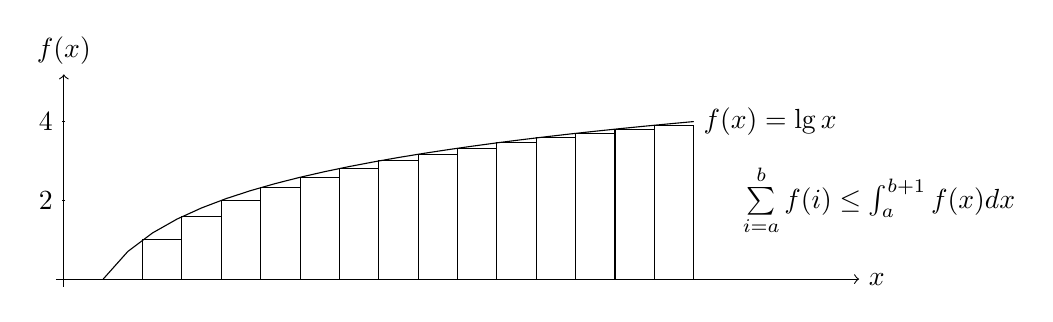
\begin{tikzpicture}[scale=0.5, domain=1:16]
            \draw[->] (-0.2,0) -- (20.2,0) node[right] {$x$};
            \draw[->] (0,-0.2) -- (0,5.2) node[above] {$f(x)$};
            \draw (1pt,2cm) -- (-1pt, 2cm) node[anchor=east] {$2$};
            \draw (1pt, 4cm) -- (-1pt, 4cm) node[anchor=east] {$4$};
            \draw[color=black] plot (\x, {ln(\x)/ln(2)}) node[right] {$f(x) =\lg x$};

            \foreach \x in {2, ..., 15}
                \draw (\x,0) rectangle (\x+1, {ln(\x)/ ln(2)});
            \draw (17, 2) node[right]{$\sum\limits_{i=a}^b f(i) \leq \int_a^{b+1} f(x)dx$};
        \end{tikzpicture}
        \label{Fig:MonotoneFunction_A}
        }
    \hfil
    \subfloat[Under approximation]
        {

        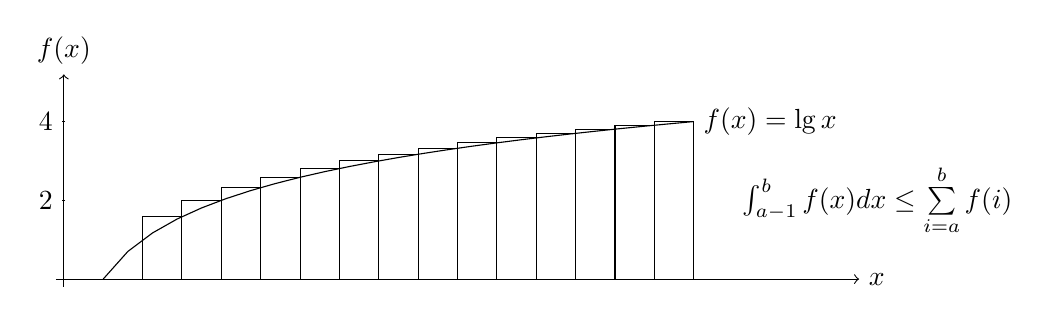
\begin{tikzpicture}[scale=0.5, domain=1:16]
            \draw[->] (-0.2,0) -- (20.2,0) node[right] {$x$};
            \draw[->] (0,-0.2) -- (0,5.2) node[above] {$f(x)$};
            \draw (1pt,2cm) -- (-1pt, 2cm) node[anchor=east] {$2$};
            \draw (1pt, 4cm) -- (-1pt, 4cm) node[anchor=east] {$4$};
            \draw[color=black] plot (\x, {ln(\x)/ln(2)}) node[right] {$f(x) =\lg x$};

            \foreach \x in {2, ..., 15}
                \draw (\x,0) rectangle (\x+1, {ln(\x+1)/ ln(2)});
            \draw (17, 2) node[right]{$\int_{a-1}^b f(x)dx \leq \sum\limits_{i=a}^b f(i)$};
        \end{tikzpicture}
        \label{Fig:MonotoneFunction_B}}
    \caption{单调递增函数的和近似}
    \label{Fig:MonotoneFunction}
\end{figure*}


\begin{example}
估计$\sum_{i=1}^n \frac{1}{i}$

\begin{displaymath}
    \sum_{i=1}^n \frac{1}{i} \leq 1+ \int_1^n \frac{dx}{x} =1 +
    \ln(x)|_1^n = 1+\ln n -\ln 1 =\ln(n) +1
\end{displaymath}
使用等式\ref{Equa:MonotonyFunction}得到。注意我们分开了和的第一项,对
剩下的部分进行了微分近似。避免了积分下限的除0运算。类似的
\begin{displaymath}
    \sum_{i=1}^n \frac{1}{i} \geq \ln(n+1)
\end{displaymath}
参见等式\ref{Equa:HarmonicSeries}取得的更接近的近似。
\end{example}

\begin{example}
$\sum_{i=1}^n \lg i$ 的下界

\begin{displaymath}
    \sum_{i=1}^n \lg i =0 + \sum_{i=2}^n \lg i \geq \int_1^n \lg xdx
\end{displaymath}
使用等式\ref{Equa:MonotonyFunctionA}(参见图\ref{Fig:MonotoneFunction_B})。
\begin{displaymath}
    \begin{aligned}
        \int_1^n \lg xdx &=\int_1^n (\lg e)\ln xdx=(\lg e)\int_1^n \ln xdx\\
        &=(\lg e)(x\ln x -x)|_1^n=(\lg e)(n\ln n -n+1)\\
        &=n\lg n -n\lg e +\lg e \geq n \lg n -n\lg e
    \end{aligned}
\end{displaymath}
既然$\lg e < 1.443$

\begin{equation}\label{Equa:1_18}
    \sum_{i=1}^n \lg i \geq n\lg n -1.443n
\end{equation}
\end{example}

使用前面例子的思想,但是使用更精确的数学方法,就可以推导出Stirling's
formula给出的n!的边界:
\begin{equation}
    \left(\frac{n}{e}\right)^n\sqrt{2\pi n}<n!<\left(\frac{n}{e}\right)^n\sqrt{2\pi
    n}(1+ \frac{1}{11n}) \qquad n\geq 1
\end{equation}

\subsubsection{不等式运算}
下列连接不等式的规则经常用到。
\begin{equation}
    \begin{aligned}
        &\mbox{传递性}   &\mbox{如果} A\leq B &\mbox{且} B\leq C   &\mbox{则} A\leq C\\
        &\mbox{加法}     &\mbox{如果} A\leq B &\mbox{且} C\leq D   &\mbox{则} A+C\leq B+D\\
        &\mbox{正数缩放} &\mbox{如果} A\leq B &\mbox{且} \alpha >0 &\mbox{则} \alpha A\leq \alpha B
    \end{aligned}
\end{equation}

\subsection{逻辑元素}\label{Sec:LogicElement}
逻辑是一个形式化自然语言语句的系统,他使得我们可以更精确的推理问题。最简单的
命题叫\emph{原子公式}。更复杂的命题可以使用\emph{逻辑连词}来组成。\emph{原子公式}
例如“4<3”,“4.2是一个整数”,“x+1>x”。注意一个逻辑命题不一定是真。一个正确
的证明才能显示一个命题是真。

最常用的逻辑连词是$\wedge$(与),
$\vee$(或)和$\neg$(非),也叫做布尔运算符。复杂命题的
真值,通过连词的规则从原子命题中推出。令A 和B 是逻辑命题,则
\begin{enumerate}
    \item $A \vee B$为真,当且仅当A和B都为真时。
    \item $A \wedge B$为真,当且仅当A和B其中一个为真,或都为真时。
    \item $\neg A$,当且仅当A为假时。
\end{enumerate}
另一个重要的推理连词叫“推导出(implies)”,我们用符号“$\Rightarrow$”来表示它。(也有时用
“$\rightarrow$”。)命题$A \Rightarrow
B$读作“A推导出B”,或是“如果A则B”。(注意这个命题没有“else”
子句。)“推导出”运算符可以表示成其他运算符的组合,考虑下面的等价:
\begin{equation}\label{Equa:ImplyLaw}
    A \Rightarrow B \mbox{在逻辑上等价于} \neg A \vee B
\end{equation}
这可以通过真值表来检验。

一个常用的等价变换叫\emph{DeMorgan}法则:
\begin{equation}
    \neg (A \wedge B) \mbox{在逻辑上等价于} \neg A \vee \neg B
\end{equation}
\begin{equation}
    \neg (A \vee B) \mbox{在逻辑上等价于} \neg A \wedge \neg B
\end{equation}


\subsubsection{量词}
还有一种重要的逻辑连词,\emph{量词}。符号$\exists x$
叫\emph{全称量词},读作“对于所有x”,而符号$\forall x$
叫\emph{存在量词},读作“存在x”。这两个量词可以适用于所有包含变量x
的命题。命题$\forall xP(x)$为真,当且仅当对于所有x,P(x)都为真时。
命题$\exists xP(x)$为真,当且仅当有x使得P(x)为真。最经常的,一个
普通的量词命题是条件:$\forall x(A(x) \Rightarrow B(x)$。读作“对
于所有x,A(x)成立,则B(x)也成立。”

量词命题服从变相的\emph{DeMorgan}法则:
\begin{equation}
    \forall xA(x) \mbox{在逻辑上等价于} \neg \exists x(\neg A(x))
\end{equation}
\begin{equation}
    \exists xA(x) \mbox{在逻辑上等价于} \neg \forall x(\neg A(x))
\end{equation}

有时将自然语言转换成量词命题是很麻烦的。人们说得话并不总是很有逻辑。我们需要
分清“for any x ”常常意味着“for all
x”,尽管“any”和“some”在正常语言中是可交换
的\footnote{译注:汉语中也有类似的问题}。最好的方针是,尝试重新以逻辑语言的形式阐述一句
自然语言,然后问自己是否和自然语言有同样的含义。例如,“任何(any)一个活人都必须
呼吸”,可以阐述为“对所有人x,x要活着就必须呼吸”,和“对于有些人x,x
要活着就必须呼吸”。那一个和原来的句子意义一样?

\subsubsection{否定量词命题、反例}
证明一个一般命题,说$\forall x(A(x) \Rightarrow
B(x)$是错的必要条件是什么?我们可以使用前面
提到的等价条件来阐明目标。首先要认识到没有必要证明$\forall x(A(x)
\Rightarrow \neg B(x)$。这是一个 过于严格的命题。否定的$\forall
x(A(x) \Rightarrow B(x)$是$\neg(\forall x(A(x) \Rightarrow
B(x)))$,它还可以进行一系 列逻辑变换:
\begin{equation}
    \begin{aligned}
        \neg(\forall x(A(x) \Rightarrow B(x))) &\mbox{在逻辑上等价于} \exists x\neg(A(x)\Rightarrow B(x))\\
        &\mbox{在逻辑上等价于} \exists x\neg(\neg A(x)\vee B(x))\\
        &\mbox{在逻辑上等价于} \exists x(A(x)\wedge \neg B(x))
    \end{aligned}
\end{equation}
换句话说如果我们可以找到一个x使得A(x)为真而B(x)为假,则我们就证明了
$\forall x(A(x)\Rightarrow B(x))$ 为假。象这样的x称为\emph{反例}。

\subsubsection{逆否命题(contrapositives )}
当试图证明一个命题时,经常将其转换成逻辑上的等价形式。其中的一个形式叫做\emph{逆否
命题}。$A \Rightarrow B$的逆否命题是$(\neg B)\Rightarrow (\neg
A)$。等式\ref{Equa:ImplyLaw}使得我们可以验证当一个命题为真时它的逆否命题也为真:
\begin{equation}
    A \Rightarrow B \mbox{在逻辑上等价于} (\neg B)\Rightarrow (\neg A)
\end{equation}
有时,证明命题的逆否命题,叫“反证法”,但是“反证法”有更精确的描述。"反证法"的严谨定义
在下一小节中。

\subsubsection{反证法}
假定要证明的命题的形式如$A \Rightarrow
B$。严谨的\emph{反证法}先做一个附加假设B为假即$\neg
B$,再证明B自己。这样要证明的全命题就是$(A \wedge \neg B)\Rightarrow
B$ 。下面的恒等式验证了这个方法:
\begin{equation}
    A \Rightarrow B \mbox{在逻辑上等价于} (A \wedge \neg B)\Rightarrow B
\end{equation}
在算法分析里很难遇到真正的反证法。但是练习1.21遇到了一个。大多数叫反证法的实际上
是证明的逆否命题。

\subsubsection{推理规则}
迄今为止我们看到了大量的\emph{逻辑等价}命题,或是\emph{逻辑恒等式}:一个命题是真,
当且仅当第二个命题也是真。恒等式是“可逆的”。但是很多证明使用的不可逆命题组合。要
证明的完全命题有“如果\emph{前提},则\emph{结论}”的形式。可逆的
“如果\emph{结论},则\emph{前提}”经常不是真的。逻辑恒等式在证明诸如“如果\emph{前提},则\emph{结论}”
的命题时不够灵活。在这种情况下,我们需要\emph{推理规则}。

一个推理规则是一个通用的允许我们从一套给定命题中得到新结论的模式。他可以被阐
述为“如果我们知道$B_1, \cdots , B_k$,我们可以总结出C”。这里$B_1,
\cdots , B_k$和C都是逻辑命题。这里有几个熟悉的规则:
\begin{equation}\label{Equa:ModusPonens}
    \mbox{如果我们知道} B and  B\Rightarrow C \mbox{则我们可以得到结论} C
\end{equation}
\begin{equation}\label{Equa:Syllogism}
    \mbox{如果我们知道} A\Rightarrow B and B\Rightarrow C \mbox{则我们可以得到结论} A\Rightarrow C
\end{equation}
\begin{equation}\label{Equa:RuleofCases}
    \mbox{如果我们知道} B\Rightarrow C and \neg B\Rightarrow C \mbox{则我们可以得到结论} C
\end{equation}
有些规则通过他们的希腊和拉丁名字为人所知的。等式\ref{Equa:ModusPonens}是
\emph{modus ponens}, 等式\ref{Equa:Syllogism}是\emph{syllogism},
等式\ref{Equa:RuleofCases}是\emph{rule of
cases}。这些规则不是相互独立的;在练习1.21中我们可以证明rule of
cases使用了其他规则和逻辑恒等式。


\section{分析算法和问题}
我们分析一个算法的目的是要改进它,如果可能,为在解决一个问题重到底选那一个方
法提供依据。我们使用下面的标准
\begin{enumerate}
    \item 正确性
    \item 所做工作的量
    \item 使用空间的量
    \item 简单,清晰
    \item 最优化
\end{enumerate}
我们将讨论每一个标准的尺度,并给出应用他们的几个例子。当考虑算法的最优性时,我们
将介绍建立问题最低边界复杂性的技术。

\subsection{正确性}
建立算法正确性主要有三步。第一,在任何决定一个算法是否正确的企图之前,我们必
须对“正确”有一个清晰的概念。我们需要一个清晰的命题来描述期望有效输入的特性(叫
前置条件),和处理每一个输入的结果(叫后置条件)。在输入前提条件满足,算法结束之后后置
条件也正确的话,我们尝试证明输入输出关系的命题。

算法有两个方面:要解决的问题和完成所需要的指令序列,也就是它的实现。建立方法和(或)
公式的正确性,可能只需要简单的也可能是一长串关于算法涉及方面的(例如图、排列、矩阵)引理
和定理。例如,应用高斯消元法解系统线性方程的有效性,依赖于一大堆线性代数的定理。
在本书的算法中使用的方法不是显然正确的;他们必须被定理证明。

一旦建立了方法,我们用程序实现他。如果一个算法短小,简洁很有美感,我们一般只使用非正式
的含义来使自己相信,其他的输入也会象我们期望的一样得到正确的结果。我们可能会仔细的检查
一些细节(例如循环计数器的初值和终值),以及用一个简单的例子手工演算算法。这些都不能
证明算法的正确性,但是非正式方法对于一些小的程序就足够了。更加正式的技术,比如循环不变式(loop
invariants),可能会用来验证部分程序。3.3节扩展了这个话题。

大多数写在类外面程序非常大而复杂的。为了证明大程序的正确性,我们可以尝试将程序分解比较小
的模块;这样的话,如果所有的小模块都正常的工作,那么整个程序是正确的;剩下的工作就是要证明
每一个小模块的正确性。这样只要算法和程序是以模块形式写成的,而且模块相互独立,可以分开验证,
任务就简单多了(更精确的说法是“只有这样的时候,验证正确性才是可能的”)。这是许多强壮的算法
是结构化、模块化的原因之一。本书中的大多数算法都是小片断组成的,这样我们就不必处理困难的
巨型算法的证明。

本书中,我们不总是正式的证明,有时候给出主题,或是算法中困难或复杂部分的解释。正确性是
可以证明的,尽管对于长、复杂的程序而言这是一个可怕的任务。在第三章我们将介绍一些技术来
帮助进行证明。


\subsection{所做工作的量}
如何度量一个算法的工作量?这个我们选择的度量应该能帮助我们比较解决同一个问
题的两个算法,这样我们就能决定到底那一个方法更有效。如果我们比较两个算法的实际执
行时间来度量两者所作工作的量将很简单,但是有很多原因使我们不能用执行时间来作为工
作的度量。首先当然是,他随使用的计算机而变化,而我们不想为一种计算机开发一种理论。
我们可以用程序执行的指令数或语句的数量来代替执行时间。他严重依赖于使用的程序设计
语言和程序员的编码风格。他还需要我们花费时间和精力为每一个要研究的算法编写调试程
序。我们想要一种工作量的度量方式,他可以告诉我们算法使用方法的效率而不依赖计算机、
程序设计语言和程序员,但也不依赖于许多具体的实现细节,比如增加循环计数器的开销、
计算数组索引以及设置数据结构指针的开销。我们的工作量度量必须足够的精确、足够的普
通,一致我们可以开发出一种可以用作许多算法和应用程序的丰富的理论。

一个简单的算法可能由许多初始化构造和循环组成。对于这样一个算法来说,循环体执
行的次数是一个公平表示工作量的好的度量方式。当然,一次循环内的工作量和其他循环
次数中可能不一样,一个算法可能有比其他算法大的循环体,但是我们只限于良好的工作量
的度量。尽管有些循环有5步而有些是9步,但循环次数巨大时,一次循环的步数就显得不重
要了。因此统计一个算法循环的次数是一个好主意。

在许多时候,为了分析一个算法,我们可以隔离出一种解决所研究问题的基本操作(或
者是算法的组成类型),忽略初始化、循环控制和其他额外开销,仅仅统计算法执行的选择
的基本操作的量。对于许多算法,每一次循环执行一次这样的操作,所以这种度量与前一段
描述的比较类似。

这里的例子是对于几个问题合理基本操作的选择:

\begin{tabular}{ll}
\hline
问题  &操作 \\
\hline
在一个数组中查找x &比较x和数组中的元素\\
两个实数矩阵相乘    &两个实数作乘法(或者是乘法和加法)\\
数组排序 &比较数组的两个元素\\
遍历一二叉树(参见\ref{Sec:BinaryTreeADT}节) &遍历边\\
任一迭代过程,包括递归 &过程调用\\
\hline
\end{tabular}

\noindent
只要选定了基本操作,就可以粗略的估计出执行基本操作的数目,我们有了一个度量算法
工作量的好标准,以及一个比较算法的好标准。这是我们在本章和其他章节中使用的方法。
你可能还是不认同这是一个好的选择;在下一节中我们将列出它合理的另一个例子。
现在,我们简单的摆出这个观点。

首先,有些情况下,我们本来就对基本操作感兴趣:可能是一个花费昂贵的比较操作,
或者可能因为一些理论上的兴趣。

其次,我们经常对随输入的增大算法所消耗时间增大的变化率感兴趣。只要得到总操作数量
和基本操作数量粗略的比例,合理的计算就可以让我们对算法对于大输入要计算多久
又一个相当清晰的概念。

最后,这种工作量的度量带了很大的灵活性。尽管我们经常选择一个或最多两个操作,我们
可以包括一些开销巨大的操作,极端的,我们可以选择特定计算机的一套指令作为基本操作。
另一种极端情况,我们可以将“一次循环”作为基本操作。因此,通过多样的基本操作的
选择方法,我们可以在分析中改变精确和抽象的程度来适应我们的需要。

如果我们为一个问题选择一个基本操作,然后发现算法指向操作的总数不与基本操作的数目
成比例,怎么办?如果基本操作的开销很大怎么办?在极端情况下,我们可能为一个特定的
问题选择了一种基本操作,然后我们发现解决这个问题的有些算法使用完全不同的操作,而
根本不使用我们要统计的操作。这时我们有两个选择。我们可以放弃关注特定的操作,转向
统计循环的次数。或者,如果我们对选择的操作特别感兴趣,我们可以将我们的研究范围
限定在适用该操作的一类算法内。对于使用与选择基本操作不同技术的其他算法,应该个别的
处理。对于一个问题的一类算法,经常通过要处理的数据的基本操作来定义。(选择
基本操作正式的程度是多样的;本书中经常使用非正式的描述。)

在这一节中,我们经常使用短语"算法所作工作的度量"。他可以用术语“一个算法的复杂性”
来代替。复杂性意味着做了多少工作,通过一些特殊的复杂性度量方式来度量,在我们大
多数的例子中是用的特定基本操作执行的数量。注意,这里复杂性与算法有多复杂多棘手无
关;一个非常复杂的算法可能有很低的复杂性。我们将使用术语“复杂性”,“工作量”和
“所作基本操作的数量”,在本书中这几个术语都是可替换的。

\subsection{平均和最坏分析}
现在我们有了分析一个算法工作量的一般方法,我们需要可以简明展示分析结果的途径。
工作量不能用一个简单数值来描述,因为对于不同的输入执行的步数不一样。我们首先
观测到工作量依赖于输入量的大小。例如,使用同样的算法,按字母排序1000个名字需要
的操作肯定比按字母排序100个名字要多。接一个12阶12元线性方程肯定解2阶2元线性方程
做的工作要多。其次,我们观察到,即使我们仅考虑一个固定的输入规模,操作执行
的数目还是可能依赖于你到底输入的是什么。如果在数组中只有少数名字不按顺序、在
前面的例子中的算法就只需要做很少的工作,但是如果数组十分混乱,就不得不做很多
的工作。如果大多数系数都是0,解一个12阶线性方程也不需要很多工作。

第一个观察指出,我们需要一种度量输入规模的标准。选一个合理的输入规模的度量通常
是很容易的。这里有一些例子:

\begin{tabular}{ll}
\hline
问题  &输入规模 \\
\hline
在名字数组中查找x   &数组中名字的个数\\
两个矩阵乘法 &矩阵的维数\\
遍历二叉树  &树节点的数量\\
解系统的线性方程 &等式的数量,或未知数的数量,或者两者\\
一个关于图的问题 &图节点的数量,或边的数量,或者两者\\
\hline
\end{tabular}

\noindent
即使输入规模固定,比如n,操作执行的数量还是依赖于到底输入了什么。那么到底
如何表示算法分析的结果呢?我们经常用\emph{最坏情况复杂性}来描述算法的行为。

\begin{definition}
最坏情况复杂性

令$D_x$ 是所考虑问题的规模为n的输入集合,I是$D_x$
的一个元素。令t(I),是对于输入I要执行的基本操作的数量。我们定义函数W
\begin{displaymath}
    W(n)=max{t(I)|I\in D_n}
\end{displaymath}
函数$W(n)$叫做算法的最坏复杂性。$W(n)$是算法对于规模为n的输入所要做基本操作的最大数量。
\end{definition}

通常计算$W(n)$是很复杂的。\ref{Sec:AsymptoticGrowthRate}节介绍了一种当精确计算
十分困难时常用的技术。最坏复杂性是很有价值得,它给出了算法所作工作量的上限。最坏分析
可以用于帮助估计一个算法特定实现的时间限制。对于本书中出现的大多数算法,我们都将进行
最坏分析。除了特别指出,当我们说一个算法的工作量时,都是指最坏情况时的工作量。

似乎更有用、更自然的描述算法行为的方法是指出他的平均工作量;就是说,计算规模为n的
所有输入的基本操作执行的数量,然后取平均。实际中一些输入出现的频率要高于其他输入,所以
带权平均更有用。
\begin{definition}
平均复杂性

令$Pr(I)$是输入I出现的概率。则算法的平均行为定义为
\begin{displaymath}
    A(n)=\sum_{I\in D_n}Pr(I)t(I)
\end{displaymath}
\end{definition}

我们通过分析算法来决定$t(I)$,但是$Pr(I)$不能通过分析计算。函数$Pr(I)$
取决于经验以及具体使用算法的应用,或者只能通过简单的假设(例如,所有情况等概率)。如果$Pr(I)$
很复杂,计算平均行为将很困难。当然,如果
依赖于使用算法的应用,函数A描述的算法的平均行为仅对该应用适用。

下面的例子展示了最坏和平均分析。

\begin{example}\label{Example:SearchInUnSortedArray}
在无序数组中查找

\emph{问题:}令E是包含n个元素的数组(关键字),$E[0],E[1] \cdots
E[n-1]$,其中元素是无序的。查找关键字为K的元素,如果K在数组中,返回索引号;
如果K不再数组中返回-1。(将在\ref{Sec:SearchInOrderArray}节中研究元素
是有序时的情况。)

\emph{策略:}依次将数组的元素与K比较,直到找到一个匹配的,或者到
达数组尾。如果K不再数组中返回-1,否则算法返回索引号。
\end{example}

有一大类过程和这个类似,我们叫这些过程为\emph{普通查找例程}。通常他们作为
复杂过程的子程序。

\begin{definition}\label{Def:GeneralSearch}
普通查找例程

\emph{普通查找例程}是一个处理不确定数量数据的过程,一直到数据处理完
或是得到目标。下面是大概的算法:

如果没有数据了:

\hspace{2ex}\emph{失败}

否则

\hspace{2ex}处理一笔数据。

\hspace{2ex}如果得到我们想要的:

\hspace{4ex}\emph{成功}

\hspace{2ex}否则

\hspace{4ex}\emph{继续处理}剩余的数据。

之所以叫\emph{普通}查找例程,是因为例程经常执行诸如查找、移动元素、增加
删除元素之类的简单操作。
\end{definition}

\begin{algorithm}\label{Algo:SequentialSearch}
顺序查找,无序的

\emph{输入:}E、n、K,这里E是一个有n个元素的数组(索引号从$0, \cdots
n-1$),$K$是要查找的条目。为了简化问题,我们假定K和E的元素都是整数,
和n一样。

\emph{输出:}返回ans,指示K在E中位置(如果K没有找到,返回-1)。
%% Todo  Fix Me
\begin{figure}
\begin{lstlisting}[language={Java},keywordstyle=\color{blue!70}, commentstyle=\color{red!50!green!50!blue!50}]
    int seqSearch(int[] E, int n, int K) {
    1   int ans, index;
    2   ans = -1;
    3   for (index = 0; index < n; ++index) {
    4       if (K == E[index]) {
    5           ans = index;
    6           break;
            }
        }
    7   return ans;
    }
\end{lstlisting}
\end{figure}

\emph{基本操作:}比较x和数组的元素。

\emph{最坏分析:}显然W(n)=n,最坏情况是在数组的最后一个元素才与K匹配的,
或者根本没有一个元素符合条件。这两种情况都将导致要比较K和所有n个元素。

\emph{平均行为分析:}我们将做一些简单的假设来分析第一个例子,稍后再以不同的假设分析
比较复杂的第二个例子。我们就假定数组中所有的元素都不相同,则如果K在数组中他将只和
其中一个元素相等。

对于我们的第一种情况,我们假设K在数组中,我们用“succ”来表示这一事件,和
\ref{Sec:Calculous}节中概率的术语保持一致。输入可以根据K到底再那里出现来分类,
所以有n个要考虑的输入。对于$0\leq i <n$,令$I_i$表示K出现在数组第i个位置的
事件。令$t(I)$为输入I时算法进行比较的次数(即程序中K=\'=E[index]的次数)。
显然对于$0\leq i <n$,$t(I_i)=i+1$。因此
\begin{displaymath}
A_{succ}(n)=\sum_{i=0}^{n-1}Pr(I_i|succ)t(I_i)=\sum_{i=0}^{n-1}(\frac{1}{n})(i+1)=(\frac{1}{n})\frac{n(n+1)}{n}=\frac{(n+1)}{2}
\end{displaymath}

脚标“succ”表示,我们假定在本次计算中完成了查找。结果符合我们平均的直觉,大约
数组的一半将被查找。

现在让我们考虑事件K不在数组中的情况,我们称为“fail”。对于这种情况只有一种输入,
我们称为$I_{fail}$ 。比较的次数$t(I_{fail})=n$,所以$A_{fail}=n$。

最后,我们结合K在数组中和K不在数组中两种情况。令q是K在数组中的概率。根据条
件期望定律(引理\ref{Lemma:ExceptionLaw}):
\begin{displaymath}
    \begin{aligned}
    A(n)&=Pr(succ)A_{succ}(n)+Pr(fail)A_{fail}(n)\\
        &=q(\frac{1}{2}(n+1))+(1-q)n=n(1-\frac{1}{2}q)+\frac{1}{2}q
    \end{aligned}
\end{displaymath}

如果$q=1$,即$K$总在数组中,则$A(n)=(n+1)/2$,和前面一样。如果$q=1/2$,即50\%的
机会$K$不在数组中,则$A(n)=3n/4+1/4$;大概要检查3/4的数组元素。这是例\ref{Example:SearchInUnSortedArray}
的结论。
\end{algorithm}

例\ref{Example:SearchInUnSortedArray}展示了我们如何解释规模为n的输入集合$D_n$。
我们仅考虑了影响算法行为的输入,即$K$在不在数组中以及K出现的位置,而不是所有可
能的名字和数组大小。$D_n$中的一个元素$I$可以认为是一个K在指定位置出现的数组
的集合(或等价类)。则$t(I)$是对于输入$I$的基本操作执行的次数。

显然,造成算法有最坏行为的输入依赖算法本身,而不是问题。对于算法\ref{Algo:SequentialSearch}
当$K$在数组的最后一个位置时,最坏情况发生。对于按逆序查找的算法(例如,
从$index=\,=n-1$开始),当K出现在数组最前面时发生最坏的情况。(另一种最坏情况发生的条件
是$K$不在数组中。)

最后,例\ref{Example:SearchInUnSortedArray}展示了在进行查找和排序的平均分析时经常
用到的假设;所有的元素都是不同的。对不同元素的平均分析给出了对重复元素较少情况的
比较接近的平均行为。如果这里有很多重复元素,就很难对K第一次出现在数组的什么地方做
出合理的假设。

\begin{example}\label{Example:MatrixMultiplication}
矩阵乘法

\emph{问题:}令$A=(a_{ij})$是一个$m\times
n$矩阵,$B=(b_{ij})$是一个$n\times
p$矩阵,两者都是实数矩阵。计算矩阵$C=AB$。(这个问题在第十二章中大量讨论。在许多
情况下,我们假设矩阵是方阵,即$m=n$,$p=n$。)

\emph{策略:}根据矩阵积的定义使用下面的算法:
\begin{displaymath}
    c_{ij}=\sum_{k=0}^{n-1}a_{ij}b_{ij} \qquad 0\leq i<m , 0\leq
    j<p
\end{displaymath}

\end{example}

\begin{algorithm}\label{Algo:MatrixMultiplication}
矩阵乘法

\emph{输入:}矩阵A和B,整数m,n,p,其中A是一个$m\times
n$矩阵,而B是一个$n\times p$矩阵。

\emph{输出:}矩阵C,$m\times p$矩阵。C被传递进来,算法填充之。

matMult(A, B, C, m, n, p)

\hspace{2ex}for(i=0; i<m; i++)

\hspace{4ex}for(j=0; i<m; i++)

\hspace{6ex}$c_{ij} = 0$;

\hspace{6ex}for(k=0; k<n; k++)

\hspace{8ex}$c_{ij}+=a_{ij}b_{kj}$


\emph{基本操作:}矩阵元素的乘法。

\emph{分析:}为了计算C的每一个元素,要做n次乘法。C有$mp$个元素,所以
\begin{displaymath}
    A(m, n, p)= W(m, n, p) = mnp
\end{displaymath}

对于$m=n=p$时,$A(n)=W(n)=n^3$。这是例\ref{Example:MatrixMultiplication}的结论。


\end{algorithm}

例\ref{Example:MatrixMultiplication}展示了有些算法只是执行指令,因此工作量
不依赖于具体的输入细节;仅依赖于输入的规模。这种情况下,最坏和平均都是一样的。
对于其他算法,就不一定了。

最坏和平均分析行为分析的概念是很有用的,即使我们选择了一种很复杂的工作量
的度量(比如,执行时间)。显然,工作量通常依赖于输入的规模和输入的特性,这使得不管
选择了什么度量的方式我们都要研究最坏和平均行为。


\subsection{空间使用}
一个程序使用的内存单元数量和执行程序所需要的时间一样,依赖于具体的实现。然而,
通过检查算法可以对空间的使用情况作出一些结论。一个程序需要存储空间来放置他的代
码、常量和程序使用的变量,以及输入的数据。还可能需要空间来操作数据,存储需要输出
的结果信息。输入数据本身可能也需要一些form,通常也需要不少空间。

如果输入数据有一个自然的形式(比如,一个数组或矩阵),则我们撇开程序和输入,
分析还需要多少额外的空间。如果额外空间的大小是一个于输入规模有关的常量,则这样的
算法称为\emph{in place}。这个属于特指排序算法。(\emph{in place}
的一个不严格定义常用于,额外空间
不为为常数的但是仅和输入规模成对数关系,原因是对数函数增长缓慢;我们会在使用不严
格定义是特别指明。)

如果输入可以表示为变量的形式,作为我们认为输入本身所需要的空间也是额外空间的
一部分。一般情况下,我们用“单元”的数量,而不对“单元”做严格的定义。你可以认为
单元足够大可以容纳一个数值或对象。如果使用的空间依赖于特定的输入,可以做最坏和平
均分析。

\subsection{简明性}
通常,但不总是,最简洁最直接解决问题的方法不是最有效的。可是算法的简明性还是
一个需要的特性。这可以更简单的验证算法的正确性。当选择一个算法时,调试一个算法的
时间也是需要考虑的,但是程序经常被使用时,它的效率将是主要的选择依据。

\subsection{最优性}
不论我们多么聪明,我们都不能将一类问题的算法性能提高的超过一个临界点。每一类
问题都有固有的复杂性,就是说要解决问题需要做的工作量有一个最小值。为了分析一个问
题的复杂性,与之对立的是我们前面讲到的分析算法的复杂性,我们选择一类算法(通常通
过算法允许执行的操作来决定)和一种复杂性的度量,例如基本操作执行的次数。之后我们
会问解决问题究竟要执行多少基本操作。如果其中有一个算法执行基本操作的次数比别的算
法都少(最坏情况),我们说这个算法是最优的(最坏情况)。注意当我们说这一类算法时,
并不意味着目前人们想到的这些算法。我们指所有可能的算法,包括还没有被发现的。“最
优”不意味着“已知最好的”, 它意味着“所有可能的最好的”。

\subsection{底限和问题复杂度}
然而我们怎么才能知道一个算法是最优的呢?我们是否必须分析所有可能的算法?(包括
一些我们目前还没有想出来的?)幸运的是,不;我们可以从理论上证明要解决一个问题执行
基本操作数的低限。然后任何算法执行的基本操作的数量都可以朝这个目标优化。因此,为了
找到一个好的算法,或换个角度说为了解决一个问题:“解决一个问题必须做的工作有多大?”,
我们必须要完成两个任务。
\begin{enumerate}
\item 设计一个看上去很有效率的算法\textbf{A}。分析\textbf{A},找到在输入规模为n时,
    \textbf{A}在最坏情况下执行基本操作的数量的函数$W_A(n)$
\item 找到一个函数F,证明对于所考虑的一类算法,在输入规模是n时,算法至少要执行
    $F(n)$步基本操作。
\end{enumerate}
如果函数$W_A(n)$与$F(n)$相等,则算法\textbf{A}是最优的(对于最坏情况)。如果不等,可能
有更好的算法或是有更好的底限。考虑,分析一个特定算法解决一个问题执行基本操作的
\emph{上限}数,以及在第2条中讲到的给出解决问题基本操作数底限(最坏情况)的理论。
在本书中,我们对于那些最优算法已知的问题,以及那些在所知的最低限和所知的最好算法
之间仍有差距得问题。下面是这两者简单的例子。

在最坏情况下算法低限的概念对于计算复杂性是十分重要的。例\ref{Example:FindMaxValueInArrary}
和\ref{Sec:SearchInOrderArray}节研究的问题以及第\ref{Sec:Chapter:Sort}章和
第\ref{Sec:Chapter:SelectionandAdversaryArguments}章将帮助你理解
低限的概念,并展示一些建立低限的技术。你必须紧记“F是一类算法的低限”的定义意味着
属于这一类的\emph{所有}算法,对于规模为n的\emph{所有}输入,算法都至少执行F(n)步基本操作。

\begin{example}\label{Example:FindMaxValueInArrary}
查找数组中最大的元素

问题:在n个元素的数组中找到最大的元素。(假设类型为\textbf{float};
当然也可以是其他类型。)

该类算法:算法可以比较合拷贝类型为float的数值,但是不能做其他操作。

基本操作:比较数组的元素和其他float类型的数据。可以是存储在其他数组中的
或是存储变量中。

上限:假设数组E中存在要找到值。下面的算法找出最大值。
\end{example}

\begin{algorithm}\label{Algo:FindMaxValue}
查找最大值

输入:E,数组,索引号从$0,\cdots n-1$;$n\geq 1$,n是数组元素的数量。

输出:返回max,E中最大的元素。

\begin{lstlisting}[language={Java}, keywordstyle=\color{blue!70}, commentstyle=\color{red!50!green!50!blue!50}]
    int findMax(E, n)
    {
        max=E[0];
        for(index=1; index<n; ++index)
        {
            if(max<index)
                max=E[index];
        }
        return max;
    }
\end{lstlisting}

在\textbf{if(max<E[index])}这一句比较数组的元素,执行了n-1次。因此
n-1是最坏情况下所作比较操作的上限值。有算法可以更少吗?

低限:为了建立低限,我们假定数组中的元素都不相同。这个假设是可行的,
因为如果我们可以为这种输入(数组的元素都不同)在最坏情况下建立低限,它
也是考虑所有输入情况下最坏行为下的低限。

在n个元素都不同的数组中,n-1个元素不是最大的。我们可以得出结论,如果一个元素
不是最大,当且仅当它至少比一个元素小。因而,n-1个元素都必须在算法中
通过比较来筛选掉。每一次比较去掉一个元素,所以至少要做n-1次比较。也就
是说,如果算法结束时还有两个或多个没有被筛选掉的元素存在,就不能肯定它
是不是最大。因此$F(n)=n-1$是要做比较次数的底限。

结论:算法\ref{Algo:FindMaxValue}是最优的,这是
例\ref{Example:FindMaxValueInArrary}的结论。
\end{algorithm}

在建立例\ref{Example:FindMaxValueInArrary}的低限中我们可能需要一些稍微不同的
观点。如果我们给出一个算法和n个元素的数组,于是算法终止并且在做少于n-1次
比较之后给出了一个结果,则我们可以证明对于某些形式的输入算法给出了\emph{错误}的
结果。如果不做多于n-2次的比较,就会有两个元素永远不会被筛选掉;也就是说
无法知道这两个元素是否比其他小。算法可以指定其中任意一个为最大元素。我们
可以简单的将另一个替换成一个比较大的数(如果必须)。既然所有比较的结果都
和前面的类似,算法给出和前面相同的结果,它将是错误的。

这个观点是逆否命题的一个证据(参见\ref{Sec:LogicElement}节)。我们证明
“如果A在任何情况下都做少于n-1次比较,则A是不正确的。”通过逆否命题,我们
可以得到结论“如果A是正确的,则A在任何情况下都要至少要做n-1次比较。”它展
示了一种对建立底限十分有效的技术,即,如果算法不做足够的工作,就可以
找到一种输入使算法得到错误的结果。

\begin{example}
矩阵乘法

问题:令$A=(a_{ij})$,$B=(b_{ij})$是两个$n \times
n$实数矩阵。计算矩阵$C=AB$;

该类算法:算法可以执行实数的乘法,除法,加法和减法。

基本操作:乘法

上限:常用的算法(参见例\ref{Example:MatrixMultiplication})做$n^3$
次乘法,因此至多需要$n^3$。

低限:有文献证明至少需要$n^2$次乘法。

结论:没有办法根据这些信息确定常用的算法是不是最优的。许多学者在努力改善低限,
证明至少需要$n^2$乘法,其他的正在寻找更好的算法。到此为止,常用的算法不是最优
的;有算法可以达到近似$n^2.376$次乘法。这个算法是最优的吗?目前低限还没有进
一步提高,所以我们不知道是否还有算法可以更低。

\end{example}

到现在为止,我们都在讨论低限和最坏情况的行为。平均行为如何呢?我们可以使用和
最坏行为一样的方法。选择一个看上去比较好的算法,位算法找到一个函数A(n),即
在输入规模为n时在平均行为下,算法要做A(n)次基本操作。然后再证明这一类算法对
于规模n的输入至少执行G(n)次操作。如果A=G,我们可以所算法的平均行为是最优的。
如果不是,继续找更好的算法或更好的低限(或者两者)。

对于许多问题分析执行操作的数量是很困难的。通常,如果一个算法执行操作的次数
在已知的最优执行次数范围之内(有时这个算法就是所知的最好的算法。),我们就认
为这个算法是最优的。在1.5节,我们将得出一种分析许多问题是否在已知的最优执行
次数范围之内,即使我们不能执行精确的分析。

我们可以使用与分析时间相同的方法来研究空间的使用。分析一个特定算法使用空间
数量的上限,在证明一个理论上的低限。我们可以认为对一个问题的算法的时间和空间
都是最优的吗?这个问题的答案是,有时是。对于许多问题存在时间和空间的平衡。

\subsection{实现和编程}
\emph{实现}就是将一个算法转换成计算机程序。算法可以通过与计算机程序设计语言类似的
操作变量和数据结构的构造来描述,或者用非常抽象的、高级的用自然语言解释解决抽象问题
的方法,不提到关于计算机的任何事物。因此实现可能是灵巧、直接的翻译工作,也可能是非常
困难的,需要程序员在选择数据结构上做很多判断。以后在适当的地方,我们将讨论在一般
情况下,实现如何选择数据结构,如何将以英语描述的算法变成程序。进行这样的的讨论有
两个原因。第一,这是生产一个好程序很自然而且重要的部分。第二,考虑实现细节对于分析
算法很必要的;在抽象对象(比如图,集合)上执行不同操作的时间依赖于对象是如何表示的。
例如,如果集合以链表表示,则连接两个集合只需要一次或两次操作。但是如果集合以数组
表示,则需要大量的操作,比如将一个集合的元素拷贝到另一个集合中。

狭义上讲,实现或简单的编程,意味着将一个算法描述细节和算法使用的数据结构转换成
一种特定计算机的程序。此时我们的分析是实现无关的(implementation-independent);
换句话说他们将独立与计算机和使用的程序设计语言,独立于算法或程序的小细节。

程序员也可以在分析算法时考虑特定计算机的信息。例如,如果不止统计一个操作,操作
可以根据执行时间建立权值;或者估计一个程序到底要执行多少秒(在最坏情况和平均情况下)。
有时使用一些具体计算机的知识将得到一个新的分析结果。例如,如果计算机有一些不寻常的、
强力的可以被高效执行的指令,则可以研究使用这些指令的一类算法,将这些指令作为操作统计。
如果计算机只有一套很有限的指令集,使得实现基本操作很低效,则要考虑不同的一类算法。
然而一般的,如果实现无关的分析做的很好。则程序依赖分析将作为一种补充。

当然考虑一种特定的实现时,也可以对算法的空间使用情况做细节分析。

任何关于问题输入的知识,都可以提高算法分析的精度。例如,如果输入仅限于所有可能输入
的一个子集,就可以只对这个子集作最坏分析。就像我们注意到的,一个好的平均行为分析
依赖于对不同输入发生概率的认识程度。


\section{简单函数的渐进增长率}\label{Sec:AsymptoticGrowthRate}
我们的度量算法工作量的方法到底如何?我们对两个算法的比较有多精确?因为我们不能
计算算法每一个步骤的执行情况,所以我们的分析必然存在不精确的因素。

假设一个问题的算法作了2n次基本操作,因而大概共有2cn次,c是某个常量,另一个算法
做4.5n次基本操作,或者共有4.5c`n.。那个运行的更快?我们确实不知道。第一个算法
可能做了许多额外的工作;就是说他的比例系数可能很高。因而如果一个函数描述的两个
算法有不同的常量因子,他可能是区别两个算法无意义的尝试(除非我们提高分析的精度)。
我们考虑在同一复杂性类中的算法。


假设一个问题的算法做$n^3/2$次乘法而另一个算法做$5n^2$。那一个算法更快呢?
对于n比较小的情况,第一个较快,但是对于n很大的情况,第二个更快--即使它做更多开销
的操作。立方函数的增长率远大于平方函数,常数因子在n变的很大时影响不大。

就像在例子中暗示的,我们希望找到一种比较简单函数的方法,能忽略常数因子和小规模
输入的。这正是我们将要研究的\emph{渐进增长率}、\emph{渐进阶}、或简单的称为函数的\emph{阶}。

它能合理的忽略常数因子和小规模输入吗?没有完全非级数、非数学的类推来帮助你理解
我们为什么使用渐进阶。假设你要选择了一个城市来居住,你的主要标准是那要有非常炎热的气候。
选择是El Paso、Texas、和Yuma、Arizona。他们之间温度差别不大,不是吗?但是要
你在三个城市间选择呢,El Paso、Yuma和Anchorage,Alaska。你肯定会马上会划去Anchorage。
这类似于两个函数有相同的阶,第三个有不同的阶。知道阶,使我们能更容易的选择;
我们可以消去离我们目标远的那些选择。

现在,在El Paso和Yuma如何选择呢(或者在两个阶一样的算法中如何选择呢)?我们可以
查看温度记录,然后找出那一个城市的平均温度比另一个城市高一点。这可以类推到比较有
相同阶的两个函数;对于算法,这表示统计所有操作,包括统计他们的精确运行时间。另一个
目的可能导致另一个标准,可能合适的工作和文化氛围是选择城市的标准,或者使用了多少
额外空间是选择算法的标准。

有一天Anchorage会比El Paso暖和吗?这是肯定的;当寒流传到El Paso时,
Anchorage很
可能有一个温暖的春天。这并不是说“一般情况下,Anchorage比El Paso要冷”是错误的。在
定义里我们将给出对于$O$,$\Theta$和其他“阶集合”函数行为的比较,将忽略n的小值。
忽略小参数(对于算法是输入规模)类似于忽略Anchorage比El Paso或Yuma要冷的少数几天。

\subsection{渐近阶的定义和符号}\label{Sec:AsymptoticOrderDefinitionAndSymbols}
我们将使用一些自然数和实数的常用记号。
\begin{definition}
自然数和实数的符号
\begin{enumerate}
    \item \emph{自然数集合}表示为$N=\{0, 1, 2, 3, \cdots\}$。
    \item 正整数表示为$N^+=\{1, 2, 3, \cdots\}$
    \item 实数集合表示为R。
    \item 正实数集合为$R^+$
    \item 非负实数的集合表示为$R^*$
\end{enumerate}
\end{definition}

\begin{figure*}[!t]
    \centering
    \begin{tikzpicture}
        \draw (0,0) ellipse (0.5cm and 1.2cm);
        \draw (0,1.2) ellipse (0.5cm and 1.2cm);
        \draw (0,0.5) node {g};
        \draw (0.2, 1.4)--(1.2, 1.4) node[anchor=west]{$\Omega(g)$:增长和$g$一样快或更快的函数};
        \draw (0.2, 0.5)--(1.2, 0.5) node[anchor=west]{$\Theta(g)$:增长和$g$一样快的函数};
        \draw (0.2, -0.4)--(1.2, -0.4)node[anchor=west] {$O(g)$:增长不如$g$快的函数};
    \end{tikzpicture}
    \caption{$\Omega$, $\Theta$, $O$}
    \label{Fig:OmegaThetaO}
\end{figure*}

令$f$和$g$是从$N$到$R^*$的函数。图\ref{Fig:OmegaThetaO}非正式的描述了我们使用
集合和函数阶之间的关系。记住这幅图,非正式的定义将帮助验证下面的正式定义和属性。

\begin{definition}
集合$O(g)$

令$g$是一个从非负整数到正实数的函数。则$O(g)$是函数$f$的集合,也是从非负整数
到正实数的,存在实数常量$c>0$和非负整数常量$n_0$,对于$n\geq n_0$,有
$f(n)\leq cg(n)$ 。
\end{definition}

\begin{figure*}[!t]
    \centering
    \begin{tikzpicture}[scale=0.5]
            \draw[->] (-0.2,0) -- (20.2,0) node[right] {$x$};
            \draw[->] (0,-0.2) -- (0,22.2) node[above] {$f(x)$};
            \draw (4cm, 1pt) -- (4cm,-1pt) node[anchor=north] {$4$};
            \draw (8cm, 1pt) -- (8cm,-1pt) node[anchor=north] {$8$};
            \draw (12cm, 1pt) -- (12cm,-1pt) node[anchor=north] {$12$};
            \draw (16cm, 1pt) -- (16cm,-1pt) node[anchor=north] {$16$};
            \draw (1pt,4cm) -- (-1pt,4cm) node[anchor=east] {$4$};
            \draw (1pt,8cm) -- (-1pt,8cm) node[anchor=east] {$8$};
            \draw (1pt,12cm) -- (-1pt,12cm) node[anchor=east] {$12$};
            \draw (1pt,16cm) -- (-1pt,16cm) node[anchor=east] {$16$};
            \draw (1pt,20cm) -- (-1pt,20cm) node[anchor=east] {$20$};
            \draw[color=black, domain=0:4] plot (\x, \x^2) node[right] {$f_1(x) =x^2$};
            \draw[color=black, domain=0:8] plot (\x, \x^2/4) node[right] {$f_2(x) =x^2/4$};
            \draw[color=black, domain=0:18] plot (\x, \x) node[right] {$f_3(x) = x$};
            \draw[color=black, domain=0:18] plot (\x, \x/4+3) node[right] {$f_4(x) =x/4+3$};
            \draw[color=black, domain=1:18] plot (\x, {ln(\x)/ln(2)}) node[right] {$f_5(x) =\lg x$};
    \end{tikzpicture}
    \caption{函数的阶是:$f_3\in O(f_4)$,
    虽然在$x>4$的时候$f_3(x)>f_4(x)$,因为这两者都是线性的。$f_1$和$f_2$有
    相同的阶。他们增长的比其他三个函数都要快。$f_5$是所展示函数中增长最慢的
    函数。}
    \label{Fig:FunctionsOrder}
\end{figure*}

将$g$作为某些\emph{给出}函数,将$f$当作我们要分析的函数是十分有用的。注意函数
$f$可能在$O(g)$内,即使对于所有$f(n)>g(n)$。重要的一点是$f$是所有$g$
\emph{乘一个常数}的上限。也就是说当n比较小的时候,不考虑f和g之间的关系。
图\ref{Fig:FunctionsOrder}展示了一些函数的阶关系。(注意图\ref{Fig:FunctionsOrder}
中的函数都是定义在$R^+$或$R^*$上连续的。描述我们将要研究算法大多数行为
的函数有许多自然的扩展。)

集合$O(g)$常读作“g的大O”,或“g的O”,尽管“oh”实际上是希腊字母omicron。
另外,尽管我们定义$O(g)$为一个集合,但实际中常说“f是g的O”,而不是
“f是g的O的一个元素”。

另外一个可选择的展示f在O(g)中的技术:
\begin{lemma}
如果$\lim\limits_{n\rightarrow \infty}\frac{f(n)}{g(n)}=c<\infty$,则$f\in O(g)$,
包含极限为0的情况。
\end{lemma}

就是说,如果$f/g$的极限存在且不是无穷,则f增长的不如g快。如果极限是无穷,f比g增长的快。

\begin{example}
有不同渐进阶的函数

令$f(n)=n^3/2$,$g(n)=37n^2+120n+17$。我们将看到$g\in O(f)$,但是$f\notin O(g)$。

既然对于$n\geq 78$,$g(n)<1f(n)$,这遵从$g\in O(f)$。我们也可以这样得到同样的结论:
\begin{displaymath}
\lim\limits_{n\rightarrow \infty}\frac{g(n)}{f(n)}=
\lim\limits_{n\rightarrow \infty}\frac{37n^2+120n+17}{n^3/2}=
\lim\limits_{n\rightarrow \infty}(74/n+240/n^2+34/n^3)=0
\end{displaymath}

我们可以通过计算$\lim f/g =\infty$,得到$f\notin O(g)$。这里有另一个可
选择的方法。我们根据一个条件假定$f\in O(g)$。如果$f\in O(g)$,则存在常数$c$和
$n_0$ 使得对于所有的$n\geq n_0$,
\begin{displaymath}
\begin{aligned}
&\frac{n^3}{2}\leq 37cn^2+120cn+17c\\
&\frac{n}{2}\leq 37c+\frac{120c}{n}+\frac{17c}{n^2}\leq 174c
\end{aligned}
\end{displaymath}

既然c是一个常数,n可以任意的大,所以不可能对于所有的$n\geq n_0$,
都有$\frac{n}{2}\leq 174c$ 。

\end{example}

当f和g在实数上是连续的不相同函数,  下面的定理对于求极限十分有用。

\begin{lemma}\label{Lemma:L'Hopital}
(L'H\^{o}pital法则)令f和g是不同的函数,分别有导数f'和g',且
\begin{displaymath}
\lim\limits_{n\rightarrow \infty}f(n)=\lim\limits_{n\rightarrow \infty} g(n)= \infty
\end{displaymath}
则
\begin{displaymath}
\lim\limits_{n\rightarrow \infty} \frac{f(n)}{g(n)} =\lim\limits_{n\rightarrow \infty} \frac{f'(n)}{g'(n)}
\end{displaymath}

\end{lemma}

\begin{example}
使用L'H\^{o}pital法则

令$f(n)=n^2$,$g(n)=n\lg n$。我们将得出$f\notin O(g)$但$g\in O(f)$。首先易得
\begin{displaymath}
\lim\limits_{n\rightarrow \infty}\frac{f(n)}{g(n)} =
\lim\limits_{n\rightarrow \infty}\frac{n^2}{n\lg n}=
\lim\limits_{n\rightarrow \infty}\frac{n}{\lg n}
\end{displaymath}
现在我们注意到(参见引理\ref{Lemma:LogFunction})符合使用
L'H\^{o}pital的条件:
\begin{displaymath}
\lim\limits_{n\rightarrow \infty} \frac{n\ln(2)}{\ln n}=
\lim\limits_{n\rightarrow \infty} \frac{\ln(2)}{1/n}=
\lim\limits_{n\rightarrow \infty}n\ln(2)= \infty
\end{displaymath}
因此$f\notin O(g)$。但$g\in O(f)$,因为无穷的倒数为0。

\end{example}

$\Omega(g)$的定义:至少增长的和g一样快的函数,这个定义是Ο(g)
\footnote{原注:计划考虑其他书和文章的读者将会注意到$\Omega$的定义有一些
小变化:短语“对于所有的”可能弱化成“对于无限多的”。$\Theta$的定义也
有类似的变化。}定义的对偶。

\begin{definition}
$\Omega(g)$集合

令g是从非负整数到正实数的函数。则$\Omega(g)$是函数f的集合,也是从
非负整数到正实数的函数,存在常数c>0,和非负整数常量$n_0$,对于所有$n\geq n_0$
都有$f(n)\geq cg(n)$
\end{definition}

另一个可选择的判断f在$\Omega(g)$方法是:

\begin{lemma}
函数$f\notin \Omega$,如果$\lim\limits_{n\rightarrow \infty}\frac{f(n)}{g(n)}>0$,
包含极限为$\infty$。
\end{lemma}

\begin{definition}
$\Theta(g)$,g的渐进阶

令g是从非负整数到正实数的函数。则$\Theta(g)=O(g)\bigcap\Omega(g)$ ,就是说,
函数集合即属于$O(g)$又属于$\Omega(g)$。“$f\in \Theta(g)$”最普通的读法是
“f是g的阶(f is order g)”。我们经常使用短语“渐进阶”,也使用术语“渐近阶复杂度”。
\end{definition}

我们也有:

\begin{lemma}
如果对于$0<c<\infty$的常数c有$\lim\limits_{n\rightarrow \infty}\frac{g(n)}{f(n)}=c$,
则函数$f\in \Theta(g)$。
\end{lemma}

\begin{example}
某些算法的渐进阶

算法\ref{Algo:SequentialSearch}(顺序查找,无序时),和算法
\ref{Algo:FindMaxValue}(查找最多的元素时)的最坏情况复杂度都是$\Theta(n)$。
算法\ref{Algo:MatrixMultiplication}(最坏和平均时)矩阵乘法的复杂度在$m=n=p$时
是$\Theta(n^3)$。
\end{example}

讨论阶集合的术语通常是不精确的。例如:“这是一个阶$n^2$算法”实际上意味着描述
这个算法行为的函数在$\Theta(n^2)$中。练习中列举了常用的几个阶集合,以及他们之间
的关系,比如$n(n-1)/2\in \Theta(n^2)$。

有时我们希望指出一个函数的渐进阶精确的比一个函数小或大。我们可以使用下面的定义。

\begin{definition}\label{Def:LittleoAndomega}
集合$o(g)$和$\omega(g)$

令g是一个从非负整数到正实数的函数。
\begin{enumerate}
\item $o(g)$是函数f的集合,也是从非负整数到正实数的函数,
$\lim\limits_{n\rightarrow \infty}\frac{g(n)}{f(n)}=0$。
\item $\omega(g)$是函数f的集合,也是从非负整数到正实数的函数,
$\lim\limits_{n\rightarrow \infty}\frac{g(n)}{f(n)}=\infty$。
\end{enumerate}
\end{definition}

一般情况,“$o(g)$”和“$\omega(g)$”读作“g的小oh”和“g的小omega”。
这常常记忆为在函数$o(g)$中的函数“小于”在$O(g)$中的函数。但是,
$\omega(g)$就不是很自然了,因为在$\omega(g)$中的函数可能大于在
$\Omega(g)$中的函数!$o(g)$更多的属性,参见练习1.33和1.34。

\subsection{渐进阶的重要性}
\begin{table}
\begin{tabular}{rccccc}
    \hline
    算法  &1 &2 &3 &4 &  \\
    时间函数(微妙)& $33n$ & $46n\lg n$ & $13n^2$ & $3.4n^3$  &$2^n$ \\
    \hline
    输入规模(n)&  \multicolumn{5}{c}{解决时间} \\
    \hline
    10     &0.00033sec  &0.0015sec  &0.0013sec  & 0.0034sec  & 0.001sec\\
    100    &0.003sec    &0.03sec    &0.13sec    &3.4sec      &$4*10^16$yr\\
    1000   &0.033sec    &0.45sec    &13sec      &0.94hr      &      \\
    10000  &0.33sec     &6.1sec     &22min      &39days      &      \\
    100000 &3.3sec      &1.3min     &1.5days    &108yr       &      \\
    \hline
    允许的时间  &  \multicolumn{5}{c}{最大解决的输入规模(大概)} \\
    \hline
    1sec    &30000    &2000  &280   &67  &20  \\
    1min    &1800000  &82000 &2200  &260  &26\\
    \hline
\end{tabular}
\caption{函数增长的速度}
\label{Table:GrowthRateOfFunction} \centering
\end{table}

表\ref{Table:GrowthRateOfFunction}
\footnote{原注:这张表(除了最后一列)和表\ref{Table:AsymptoteOrder}
根据Jon Bentley的《Programming Pearls》(Addison-Wesley, Reading,Mass.,1986)
改编,得到授权。}展示对于同一个问题几种实际算法的运行时间。
(最后一列不对应任何问题的算法;在这里用它来证明指数函数增长的多么快,以及指数
算法是如何的糟糕。)纵观整个表,可以看出对于复杂性很高的算法,在输入规模增长时
所消耗的时间急剧增加。表中的一个重要的经验即使是在输入很小的时候,$\Theta(n)$
和$\Theta(n\log n)$的大常数因子也不会使得他们比其他算法要慢。

\begin{table}
    \centering
    \begin{threeparttable}
    \begin{tabular}{rcc}
        \hline
        &Cray-1 Fortran\tnote{a} &TRS-80 Basic\tnote{b} \\
        n  & $3n^3 纳秒$  & 19,500,000n 纳秒\\
        \hline
        10 &3微妙 & 0.2秒\\
        100 &3毫秒 & 2.0秒\\
        1000 & 3秒 & 20秒\\
        2500 & 50秒 &50秒\\
        10000 & 49分钟 & 3.2分钟\\
        1000000 & 95年  &5.4小时\\
        \hline
    \end{tabular}
    \begin{tablenotes}
        \item [a] Cray-1是Cray Research公司的商标
        \item [b] TRS-80是Tandy公司的商标
    \end{tablenotes}
    \caption{渐进阶胜出}
    \label{Table:AsymptoteOrder}
    \end{threeparttable}
\end{table}

表的第二部分显示出了不同的增长率,在输入规模增大情况下所消耗的计算时间(当然
你可以使用更快的计算机来求计算时间)的不同。一般情况下,并不是我们多计算60倍
的时间(或者把速度提高60倍),就可以多处理60倍的输入;这种情况仅当算法的复杂性
为$O(n)$时才成立。例如对于$\Theta(n^2)$ 的算法,仅能多处理$\sqrt{60}$倍的输入。

为了进一步显示当输入规模很大时,渐进阶对时间造成的影响要比常数因子更重要,
参考表\ref{Table:AsymptoteOrder}。表\ref{Table:GrowthRateOfFunction}中的一个
立方算法在Cray-1超级计算机上实现;对于规模为n的输入要运行$3n^3$纳秒。线性
算法在TRS-80(80年代便宜的PC);要运行19.5n微秒(19,500,000n纳秒)。尽管线性
算法的常数因子比立方算法的常数大650万倍,当输入$n\geq 2500$时线性算法还是要快。
(到底是大输入还是小输入倚赖于具体的问题)。

如果我们关注函数的渐进阶(因而说n和1,000,000n是同一个类型),则当我们说两个
函数有不同阶时,我们是在强调描述这两个算法的函数的不同。如果两个函数有相同
的阶,他们可能在大常数因子上有差别。但是,现在的问题是在给定的时间内在更
快速的计算机上一个算法能处理最大的输入规模,常数的值是不相干的。就是说,
在对于表\ref{Table:GrowthRateOfFunction}的最后两行,常数的值和增长不相干。
让我们更仔细的观察这些数字的含义。

\begin{table}
\centering
\begin{tabular}{ccc}
    \hline
    对于输入规模n执行步数 & 最大可能的输入规模  &最大可能输入规模\\
    &  &增加t倍时相应的时间\\
    $f(n)$  &$s$  &$s_{new}$\\
    \hline
    $\lg n$  & $s_1$  & $s_1^t$\\
    $n$      & $s_2$  & $ts_2$\\
    $n^2$    & $s_3$  & $\sqrt{t}s_3$\\
    $2^n$    & $s_4$  & $s_4+\lg t$\\
    \hline
\end{tabular}
\caption{在最大输入规模确定时增加计算机速度得到的效果}
\label{Table:EffectOfUseFasterComputer}
\end{table}

假设,我们固定一定量的时间(一秒,一分钟--具体是多少并不重要)。令
s为特定算法在给定时间之内的能处理的最大输入规模。现在假设我们允许t倍
的时间(或者我们计算机的速度增加t倍,或者是因为技术的进步,或者
只是因为我们过时了于是买一个更贵的机器)。表\ref{Table:EffectOfUseFasterComputer}
展示了几种不同复杂性对加速的影响。

在第3列的值根据下列公式计算
\begin{displaymath}
f(S_{new})=\mbox{加速之后的步数}=t*\mbox{加速前的步数}=tf(s)
\end{displaymath}
\noindent
和$S_{new}$的关系
\begin{displaymath}
f(S_{new})=tf(s)
\end{displaymath}

现在,如果我们将第一列的函数乘以常数c,在第三列的值不会改变!这就是
我们说常数的值与输入为算法能处理的最大输入规模时增加计算时间
(或速度)产生的效果无关。


\subsection{O $\Omega$和$\Theta$的属性}
渐进阶由许多有用的属性。大多数的证明都留到练习中;他们都可以从
定义从轻松得到。对于所有的属性,假定f、g、h符合$N \rightarrow R^*$
。就是说,函数都是从非负整数到非负实数的。

\begin{lemma}
如果$f\in O(g)$以及$g \in O(h)$,则$f\in O(h)$
;就是说,Ο是传递的。同时,$\Omega$、$\Theta$、$o$和$\omega$都是传递的。

\emph{证明:}令$c_1$和$n_1$对于所有的$n \geq n_1$,都有$f(n)\leq c_1g(n)$。
令$c_2$和$n_2$对于所有的$n\geq n_2$,都有$g(n)\leq c_2h(n)$。则对于所有的
$n\geq max(n_1, n_2)$,$f(n)\leq c_1c_2h(n)$。所以$f\in O(h)$
。对于$\Omega$、$\Theta$、$O$和$\omega$的证明类似
\end{lemma}

\begin{lemma}\mbox{}\par
\begin{enumerate}
\item 当且仅当$g \in \Omega(f)$时,$f\in O(g)$。
\item 如果$f\in \Theta(g)$,则$g\in \Theta(f)$。
\item $\Theta$定义了一种函数的等价关系(参见\ref{Sec:Relationship}小节)。
        每一个$\Theta(f)$都是可以称为复杂类的等价类。
\item $O(f+g)=O(\max(f,g))$  。对于$\Omega$和$\Theta$也有同样的
        等式。(在分析复杂算法的时候他们是很有用的,这时f和g可能描述
        的算法的不同部分。)
\end{enumerate}
\end{lemma}

既然$\Theta$定义了一种等价关系,我们可以通过类中的任意函数来表示算法的
复杂性类。经常选择最简单的表示。因此如果一个通过函数$f(n)=n^3/6+n^2+2\lg n +12$
描述的算法,我们简单的说:算法的复杂性在$\Theta(n^3)$。如果$f\in \Theta(n)$,
我们说f是线性的;如果$f\in \Theta(n^2)$,我们说f是平方的;如果$f\in \Theta(n^3)$,
我们说f是立方的\footnote{原注:注意术语线性、平方和立方比他们在数学上的用法要宽松}。
$O(1)$表示函数以常量为边界(对于大的n)。

这里有两个有用的定例。他们的证明用到了在\ref{Sec:AsymptoticOrderDefinitionAndSymbols}
小节中提到的技术,特别是L'H\^{o}pital法则;证明留到练习中了。

\begin{lemma}
$\lg n$对于任意$\alpha>0$都在$o(n^\alpha)$内。就是说对数函数比正指数的幂函数都要慢
(包括指数为分数的情况)。
\end{lemma}

\begin{lemma}
$n^k$对于任意$k>0$都在$o(2^n)$内。就是说,幂函数比指数函数$2^n$要慢。
(事实上,当指数函数的底大于1时,幂函数比指数函数要慢)。
\end{lemma}

\subsection{渐进阶的和}
阶符号使我们可以容易的导出和记住在分析算法中遇到的各种渐进阶的和。有些求和结论
在\ref{Sec:Calculous}中定义。

\begin{figure*}[!t]
    \centering
    \subfloat
        {
        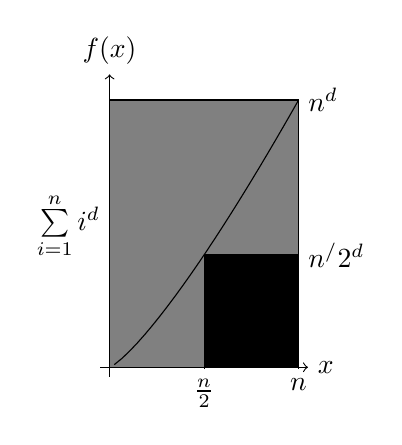
\begin{tikzpicture}[scale=0.6]
            \draw[->] (-0.2,0) -- (4.2,0) node[right] {$x$};
            \draw[->] (0,-0.2) -- (0,6.2) node[above] {$f(x)$};
            \draw (2cm, 1pt) -- (2cm,-1pt) node[anchor=north] {$\frac{n}{2}$};
            \draw (4cm, 1pt) -- (4cm,-1pt) node[anchor=north] {$n$};
            \filldraw[fill=gray] (0,0) rectangle (4,{4^1.25});
            \draw[color=black, domain=0.1:4] plot (\x, {\x^1.25}) node[right] {$n^d$};
            \filldraw[fill=black] (2,0) rectangle (4,{2^1.25});
            \draw (4,{2^1.25}) node[right]{$n^/2^d$};
            \draw (0, 3) node[left]{$\sum\limits_{i=1}^n i^d$};
        \end{tikzpicture}
        }
    \hfil
    \subfloat
        {
        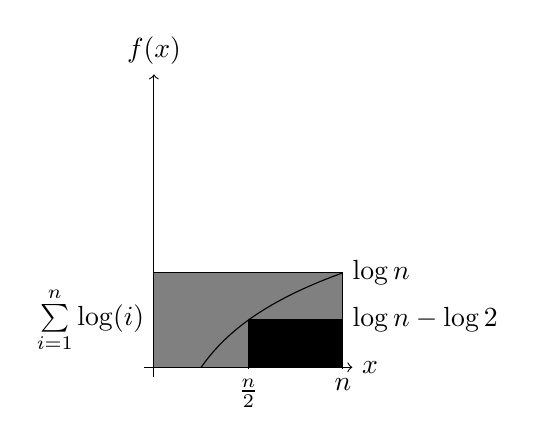
\begin{tikzpicture}[scale=0.6]
            \draw[->] (-0.2,0) -- (4.2,0) node[right] {$x$};
            \draw[->] (0,-0.2) -- (0,6.2) node[above] {$f(x)$};
            \draw (2cm, 1pt) -- (2cm,-1pt) node[anchor=north] {$\frac{n}{2}$};
            \draw (4cm, 1pt) -- (4cm,-1pt) node[anchor=north] {$n$};
            \filldraw[fill=gray] (0,0) rectangle (4,2);
            \draw[color=black, domain=1:4] plot (\x, {ln(\x)/ln(2)}) node[right] {$\log n$};
            \filldraw[fill=black] (2,0) rectangle (4,1);
            \draw (4,1) node[right]{$\log n - \log 2$};
            \draw (0, 1) node[left]{$\sum\limits_{i=1}^n \log(i)$};
        \end{tikzpicture}
        }
    \caption{矩形提供了许多和的上界和下界。当两个矩形的区域都有同样的渐进阶时,就是和的渐进阶。}
    \label{Fig:MatrixOfUpDownBound}
\end{figure*}

\begin{theorem}\label{Theorem:1_13}
令d非负常量且令r是一个不对于1的正常量。
\begin{enumerate}
\item \emph{多项式级数}的和将指数增加1。度为d的\emph{多项式级数}的和有
        $\sum\limits_{i=1}^{n}i^d$的形式,应用规则得这种形式的和在
        $\Theta(n^{d+1})$内。
\item \emph{几何级数}的和在最大一项的$\Theta$之内。\emph{几何级数}的和有
        $\sum\limits_{i=a}^{b}r^i$ 的形式。

        规则适用于0<r<1或r>1的情况,但是在r=1是是不一定的。界限a和b不能都是
        常量;典型的,上界b是n的某个函数,下界a是一个常量。
\item 对数级数的和在$\Theta(最大项)$。对数级数的和有$\sum\limits_{i=1}^{n}\log(i)$
        的形式。使用规则得到和在$\Theta(n\log(n))$内。式子中对数的底是
        多少关系不大。
\item 多项式-对数级数的和,有$\sum\limits_{i=1}^{n}i^d\log(i)$的形式,在
        $\Theta(n^{d+1}\log(n))$ 。
\end{enumerate}

证明:看图\ref{Fig:MatrixOfUpDownBound}。既然引理中所有的序列都有
$\sum\limits_{i=1}^nf(i)$的形式,这里$f(i)$是单调的。很显然,高为$f(n)$,宽为n的
大矩形是和的上界。同时,如同在图\ref{Fig:MonotoneFunction_B}中看到的,$i=0$
到$i=n$之间的在$f(i)$之下的图的面积是和的下界。对于多项式和对数序列的情况,面积
可以简单的由下面比较小的灰矩形界定。在左边的图中大矩形的面积是$n^{d+1}$ ,而
小矩形的面积是$n^{d+1}/2^{d+1}$ 。既然两个矩形的面积有同样的渐进阶,则和也
应该是这个阶。在右边的图中,两个是$n\log n$和$(n/2)(logn-log2)$。多项式-对数级数
是类似的,但是这个技术不能用于几何级数。几何序列的规则可以直接由\ref{Sec:Calculous}
节的等式\ref{Equa:ArithmeticGeometrySeries}得出。

\end{theorem}

\section{在有序数组中查找}\label{Sec:SearchInOrderArray}
为了阐明前面章节中展现的观点,我们将学习一个熟悉例子。
\begin{problem}
有序数组查找

给出包含n个有序元素的数组E,给出值K,作出索引index,K=E[index],或者K不在数组中则返回-1。
\end{problem}
实际中,K常常是条目的关键字,条目是一个除了关键字域还带其他实例域
的类,所以更精确的表述应该是K=E[index].key。为了方便讨论,我们假定条目
就是关键字,而且他们是一些数字。

让我们先假装不知道二分查找算法(Binary
Search),就像我们第一次可看到这个问题一样。我们将考虑不同的算法,分析
最坏和平均行为,最后考虑二分查找,并且通过建立需要进行关键字比较的低限
来展示二分查找是最优的。

\subsection{一些解决方法}
显然顺序查找算法(算法\ref{Algo:SequentialSearch})可以解决问题,但是
它没有使用数组元素是有序这一事实。我们能否修改算法使之使用增加的额外
信息而减少工作量呢?

第一项改进通过观察可以迅速得到,既然数组是递增的,则一旦找大于K的元素,
算法就可以结束并返回-1了。(必须如何修改算法的第4行的测试以避免在一次
循环中进行两次比较?)这个改变对分析有何影响呢?无疑,修改过的算法对于
有些情况更好;对于有些输入迅速的终止了。但是,在最坏情况下结果不变。
如果K是数组的最后一个元素,或者K是最大的元素,则算法还是要进行n次比较。

对于平均情况分析,我们必须知道K在两个数组元素\emph{之间}的可能性由多大。假设
我们定义一个间断(gap)$g_i$,是y的集合,$E[i-1]<y<E[i](i= 1, \cdots,n)$。
令$g_0$是所有比E[0]小的元素的集合,$g_n$是所有比E[n-1]大的元素的集合。
我们假定,就像我们在例\ref{Example:SearchInUnSortedArray}中做的,K在数组
中的概率是q。如果K在E中,我们假定K在所有位置的概率都是一样的(也就是有
条件概率$1/n$)。如果K不在数组中,我们假定所有的间断都是相等的(也就是有
条件概率$1/(n+1)$)。对于$0\leq i <n$,需要进行i+1次比较来决定K=E[i]或
是K在$g_i$中,而且将进行n次比较来确定K在$g_n$中。我们计算比较的平均
次数,有条件的成功$(A_{succ})$和有条件的失败$(A_{fail}))$,如下:
\begin{displaymath}
\begin{aligned}
&A_{succ}(n)=\sum_{i=0}^{n-1}\left(\frac{1}{n}\right)(i+1)=\frac{n+1}{2}\\
&A_{fail}(n)=\sum_{i=0}^{n-1}\left(\frac{1}{n+1}\right)(i+1)+\left(\frac{1}{n+1}\right)
\end{aligned}
\end{displaymath}
\noindent
第一个等式展示了K在数组中的情况,与例\ref{Example:SearchInUnSortedArray}中的
相同。第二个等式展示了K不在数组中的情况。估计和很简单,留到了练习中。
就像在例\ref{Example:SearchInUnSortedArray}中一样,最后的结果通过等式
$A(n)=qA_{succ}(n)+(1-q)A_{fail}(n)$计算。A(n)粗略的结果是n/2,不管q是
多少。当q=1/2时算法\ref{Algo:SequentialSearch}平均要比较3n/4的元素,
所以修改后的算法有改进,尽管它的平均行为还是线性的。

Let's try again. 我们能否找到一种在最坏情况下也小于n次比较的算法呢?
假设我们将K与数组中每个第4个元素比较。如果匹配,就成功了。如果K比进行比较
的元素大,即E[i],则三个在E[i]前面的元素就不用比较了。如果K<E[i],
则K在最后比较的两个元素之间。再有几次比较(是多少?)就可以决定K的
位置了如果K在数组中,或者决定K不在数组中。算法的细节和分析留给读者去
完成,但是很容易看到只有1/4的数组元素被检查到了。即使在最坏情况下也
只做大约n/4次比较。

我们可以使用同样的方法,选择一个大值j并且设计一种算法,只需要将K与1/j的
元素进行比较,因此在我们处理数组时允许每次比较消除j-1个元素。因而我们
在E中确定一个可能包含K的小段大概需要进行n/j次比较。则我们继续用进行j次
比较就能在小段中找到K。对于一个固定的K算法仍然是线性的,但是如果我们
选择j为(n/j+j)的最小值,这个值应该是$\sqrt{n}$。此时总的比较次数仅为
$2\sqrt{n}$ 。我们突破了线性的屏障。

但是我们还可以做的更好吗?注意我们在定位了小段之后继续使用线性策略。
段有大约j个元素,然后我们花了j次比较来搜索他,这个过程是线性的。但是
现在我们知道线性消耗太高了。这建议我们在小段上递归的使用我们的
“主策略”,代替线性策略。

著名的二分查找算法的想法就是将“每1/j的元素”应用到每一步中,在每次
跳过一半的元素。不用选择一个特定的整数j,不用将K与每1/j元素比较,我们
首先将K与数组正中间的元素相比较。这样在一次比较中就排除了一半的元素。

一旦我们决定了那一半可能包含K,我们递归的应用策略。我们继续比较K和剩下
段正中间元素比较,直到可能包含K的段缩小到0或者找到K。每一次比较之后
可能包含K的段会减少一半。注意,这是一个普通搜索例程的另一个例子
(定义\ref{Def:GeneralSearch})。当可能包含K的段收缩到0时,过程失败;
如果找到K则\emph{成功};两者都没有发生时\emph{继续搜索}。

这个过程是\emph{分而治之}策略的主要例子,我们将在第
\label{Sec:Chapter:RecursionAndInduction}和第\ref{Sec:Chapter:Sort}章
讨论这个策略。通过将K与正中间元素的比较,将在n个排序元素中查找K的问题
分成了两个子问题(假定正中间的元素不是K)。通过分析我们将看到分开解决
两个子问题比解决原来没有分开的问题要简单(在最坏情况和平均情况下)。事
实上,其中一个子问题不需要解决,因为我们已经知道K不在数组的那部分中。

\begin{algorithm}\label{Algo:BinrarySearch}
二分查找

输入:E,first,last和K,这里E是一个在范围$first,\cdots,last$之间顺序
的数组,K是待查找的关键字。为了简化问题,我们假定K和E的元素都是整数,
和first和last一样。

输出:index,如果K在E中,E[index]=K,如果K不在E中index=-1。
\begin{figure}
\begin{lstlisting}[language={Java}, keywordstyle=\color{blue!70}, commentstyle=\color{red!50!green!50!blue!50}]
    int binarySeach(iny[] E, int first, int last, int K)
    {
1       if(last<first)
2           index=-1;
3       else
        {
4           int mid= (first+last)/2;
5           if(K==E[mid])
6               index=mid;
7           else
            {
7               if(k<E[mid])
8                   index=binarySearch(E,first,mid-1,K);
9               else
10                  index=binarySearch(E,mid+1,last,K);
            }
        }
11      return index;
    }
\end{lstlisting}
\end{figure}

\end{algorithm}

算法\ref{Algo:BinrarySearch}正确性的详细证明在介绍了一些必须的材料之后,
在\ref{Sec:ParadigmOfSingleAssignment}节中作为一个正式例子给出。这种
经常使用的不正式的原因在前面讨论过了。

\subsection{二分查找的最坏情况分析}
让我们定义二分查找的大小n=last-first+1,E中要查找元素的数量。对二分查找
的基本操作的合理原则是K与数组元素的一次比较。(这里讨论的“比较”总是
意味着一次K与数组元素的比较,而不是第一行中index 的比较。)令W(n)为查找n
个元素数组的时要做的比较的数目。

通常假设比较都是3元比较,就像在第5和第7行进行的。(即使不进行3元比较,用
二元比较也可以达到相同的边界,见练习1.42。)因此,W(n)也是调用binarySearch
的次数, 除了在第2行没有比较就结束的情况。

\textit{Java语言提示:}许多Java的许多类,包括\textbf{String},通过
\textbf{Comparable}接口支持三元比较;用户定义类也可以实现这个接口;
参见附录A。

假设n>0。算法的任务是从first到last的n个元素中找出K。它在第5行将K与E[mid]
比较,$mid=\lfloor(first+last)/2\rfloor$ 。在最坏情况下,这些关键字都不
相等,到达第8行或是第10行,取决于到底是左边还是右边的段包含K。有多少元素
在剩下的段中呢?如果n是偶数,则有n/2个元素在右边的段中,有(n/2)-1个元素
在左边的段中。如果n是奇数,两边的段中都有(n-1)/2个元素。因此,在每次递归
之前还有$\lfloor n/2\rfloor$个元素在剩下的段中。因此保守估计在每次递归调用
之后范围被缩小一半。

我们要将n除2多少次才能使结果刚好大于1?换句话说,对于$n/2^d\geq 1$成立的
d的最大值?求解d:$2^d\leq n$和$d\leq \lg(n)$。因此在递归调用之后我们能
做$\lfloor\lg(n)\rfloor$次比较,在递归调用之前还有一次,总共需要做
$W(n)=\lfloor\lg(n)\rfloor+1$次比较。练习1.5给出这个表达式更简明的表达式,
而且对于n=0的情况也能很好的适应,$\lceil\lg(n+1)\rceil$。我们有:

\begin{theorem}
在最坏情况下二分查找算法需要将K与数组的元素进行$W(n)=\lceil\lg(n+1)\rceil$
次比较(这里$n\geq 0$,是数组元素的数目)。由于每个函数调用做一次比较,
运行时间在$\Theta(\log n)$。
\end{theorem}

在最坏情况下,二分查找平均要比顺序查找做的比较少。

\subsection{平均情况分析}

\begin{table}
    \centering
\begin{tabular}{cccccc}
\hline
    $i$ & $t(I_i)$  &   &   &$i$  & $t(I_i)$ \\
    \hline
    0   &4  & &            &13  & 4\\
    1   &5  & &            &14  &5 \\
    2   &3  & &            &15  &3 \\
    3   &4  & &            &16  &4 \\
    4   &5  & &            &17  &5 \\
    5   &2  & &            &18  &2 \\
    6   &4  & &            &19  &4 \\
    7   &5  & &            &20  &5 \\
    8   &3  & &            &21  &3 \\
    9   &5  & &            &22  &5 \\
    10  &4  & &            &23  &4 \\
    11  &5  & &            &24  &5 \\
    12  &1  & &            &间断25,28,31,38,41,44   &4 \\
        &   & &            &其他间断    &5\\
\hline
\end{tabular}
\caption{n=25时,二分查找进行比较的数量与K位置的关系}
\label{Table:BinrarySearchCompareCount}
\end{table}

为了简化分析,我们假定K可能出现在数组的任何地方。就像我们在本节开始时看到的,
有2n+1个位置K可能出现:E中的n个位置称为\emph{成功位置},n+1个间断成为
\emph{失败位置}。对于$0\leq i <n$,令$I_i$表示在K=E[i]时的所有输入。
对于$1\leq i <n$ ,令$I_{n+1}$ 表示$E[i-1]<K<E[i]$时的所有输入。$I_n$和
$I_{2n}$分别表示$K<E[0]和K>E[n-1]$时的输入。令$t(I_i)$为在输入$I_i$时算法
进行K与数组元素比较的数量。表\ref{Table:BinrarySearchCompareCount}展示了
n=25时t的值。显然大多数成功的和所有间断都在最坏情况内;大多数时候只要进行
4或者5次比较。(对于n=31我们将发现大多数成功的和所有的间断都刚好等于最坏
情况。)所以我们假设所有成功的位置都是相等的,肯定可以期望比较次数的平均值
接近与$\lg n$。计算平均值时假定每一个位置有1/51的概率时比较次数是223/51,
或者大约是4.37,$\lg 25\approx 4.65$。

既然比较的平均次数依赖于查找成功的概率,我们用q表示概率,定义$A_q(n)$为当成功
的概率是q时比较的平均次数。由条件概率法则我们有
\begin{displaymath}
A_q(n)=qA_1(n)+(1-q)A_0(n)
\end{displaymath}
\noindent
因此我们可以在特定情况的分别解出$A_1(n)$(正中间成功)和$A_0(n)$(正中间
失败),合并他们就可以得到一个适用于所有q的结果。注意$A_1$等同$A_{succ}$,
$A_0$等同于$A_{fail}$,后者是在顺序查中使用的术语。

我们将推导$A_0(n)$和$A_1(n)$的近似公式,给出下列假设:
\begin{enumerate}
\item 所有成功位置都近似相等:$Pr(I_i|succ)=1/n$,对于所有的$1\leq i \leq n$
\item $n=2^k-1$,对于所有的整数$k\geq 0$
\end{enumerate}
后一个假设是为了简化分析。所有n的结果和我们将得到的结果非常接近。

至于让$n=2^k$是想让每次失败的查找都刚好使用k次比较,不管K在那个间断中。因此
$A_0(n)=\lg(n+1)$。

分析成功查找平均行为的关键是做一个转换,即将“对于一个特定的输入$I_i$
要进行多少次比较?”转换成“多少输入需要做t次比较?”。对于$1\leq t \leq k$,
令$s_t$是使算法要做t次比较的输入数量。

例如对于n=25,$s_3=4$,因为有4个输入会做3次比较$I_2$,$I_8$,$I_{15}$和$I_{21}$。

易的$s_1=1=2^0$,$s_2=2=2^1$,$s_3=4=2^2$,以及$s_t=2^{t-1}$。既然每一个
输入都有1/n的概率,算法做t次比较的概率是$s_t/n$,由等式\ref{Equa:ArithmeticGeometrySeries}
平均是
\begin{displaymath}
A_1(n)=\sum\limits_{t=1}^{k}t\left(\frac{s_t}{n}\right)
=\frac{1}{n}\sum\limits_{t=1}^{k}t2^{k-1}=\frac{(k-1)2^k+1}{n}
\end{displaymath}
(如果我们没有假定$n=2^k-1$,$s_k$的值将不是这种样式,有些失败情况将仅有k-1次
比较,就像在表\ref{Table:BinrarySearchCompareCount}中看到的。)现在,既然$n+1=2^k$,
\begin{displaymath}
A_1(n)=\frac{(k-1)(n+1)+1}{n}=\lg(n+1)-1+O\left(\frac{\log n}{n}\right)
\end{displaymath}
就像提及的,$A_0(n)=\lg(n+1)$是K不在数组中的情况。因而我们总结出下列的引理:

\begin{theorem}
二分查找(算法\ref{Algo:BinrarySearch})对于有n个元素的数组要做大约$\lg(n+1)-q$
次比较,这里q是查找成功的概率,所有的成功位置都是相等的。
\end{theorem}

\subsection{优化}
在前一节里,我们将一个$\Theta (n)$算法改进成了一个$\Theta
(\sqrt{n})$算法,进而到了$\Theta (\log n)$。还可
以进一步改进吗?即使我们不能在提高渐进阶,我们能够改进常数因子吗?底限分析的规则
告诉我们这两个问题可能都是否定的。一个严格的底限,其中一个匹配我们算法的上限,保
证我们不能在找到改进的方法。

我们将展示二分查找算法是这类只能对数组元素做比较的算法中最优的。我们将通过检
查这类查找算法的\emph{决策树},建立一个需要比较次数的底限\footnote{原注:我们
假设读者知晓二叉树的术语,包括\emph{根},\emph{叶子}和\emph{路径};如果没有
在继续之前请提前看\ref{Sec:BinaryTreeADT}节}。令\textbf{A}是这样一个算法。
\textbf{A}的决策树和一个给定规模为n的输入是一个二叉树,二叉树的节点用0到n-1之
间的数标记,遵循下面的规则:
\begin{enumerate}
\item 树的根由算法\textbf{A}比较的第一个数组元素的索引标记。
\item 假设一个特定的节点标记为i。当算法比较K之后作左子树是K<E[i]的情况,
        右子树是K>E[i]的情况。如果算法比较之后终止了而且发现K<E[i]
        (或者K>E[i]),则这个节点没有左(或右)子树。对于K=E[i]的情况没有
        分支。一个合理的算法在这种情况下不再做比较了。
\end{enumerate}

\begin{figure*}[!t]
    \centering
    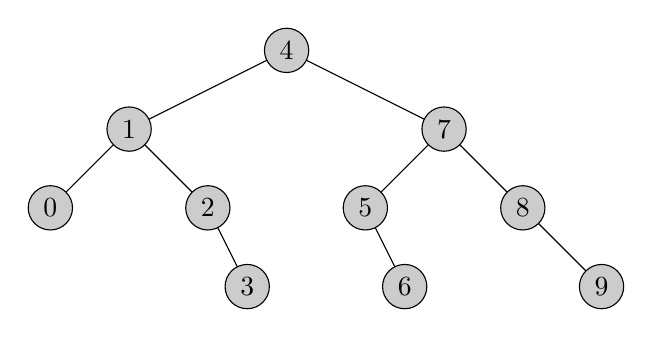
\begin{tikzpicture}
        \draw (4,3) -- (2, 2);
        \draw (4,3) -- (6, 2);
        \draw (2,2) -- (1, 1);
        \draw (2,2) -- (3, 1);
        \draw (6,2) -- (5, 1);
        \draw (6,2) -- (7, 1);
        \draw (3,1) -- (3.5, 0);
        \draw (5,1) -- (5.5, 0);
        \draw (7,1) -- (8, 0);

        \filldraw[fill=black!20!white] (4,3) circle(8pt) node{4};
        \filldraw[fill=black!20!white] (2, 2) circle (8pt) node{1};
        \filldraw[fill=black!20!white] (6, 2) circle (8pt) node{7};
        \filldraw[fill=black!20!white] (1,1) circle (8pt) node{0};
        \filldraw[fill=black!20!white] (3,1) circle (8pt) node{2};
        \filldraw[fill=black!20!white] (5,1) circle (8pt) node{5};
        \filldraw[fill=black!20!white] (7,1) circle (8pt) node{8};
        \filldraw[fill=black!20!white] (3.5,0) circle (8pt) node{3};
        \filldraw[fill=black!20!white] (5.5,0) circle (8pt) node{6};
        \filldraw[fill=black!20!white] (8,0) circle (8pt) node{9};
    \end{tikzpicture}
    \caption{n=10时二分查找算法的决策树}
    \label{Fig:BinrarySearchDecisionTreeFor10}
\end{figure*}

可以用这种决策树模型表示的算法是很广泛的;包括顺序查找和本节开始讨论的变长查找。
(注意允许算法在数组中两个关键字,但是这不提供任何信息,因为数组已经是排序的了,
所以我们不为决策树增加这种节点。)图\ref{Fig:BinrarySearchDecisionTreeFor10}展示
了n=10时二分查找算法的的决策树。

给出特定的输入,算法\textbf{A}将执行决策树中从根开始的一条路径上的所有比较。执行
关键字比较的次数就是路径上节点的个数。最坏情况下执行比较的次数就是最长的一条
路径的节点数;称这个数为p。假定决策树有N个节点。每一个节点最多有两个孩子,则在
给定深度的(counting each edge as one)节点的数目大约是前一级深度的节点数目的
两倍。既然对于所有节点到根的长度是p-1,我们有
\begin{displaymath}
N\leq 1+2+4+\cdots+2^{p-1}
\end{displaymath}
由等式\ref{Equa:PowerOf2}的右边的部分是 ,所以我们有$2^p \geq (N+1)$。

我们有了p和N的关系,但是我们想要得到p到n的关系,n是数组中要查找的元素的数目。
关键的问题是如果算法\textbf{A}在所有情况下都正确的话,$N \geq n$ 。我们需要将
决策树中一些节点用i标记,每一个i从0到n-1。

用反证法,假设有没有被标记i的节点,有些i在0到n-1的范围内。我们可以安排两个输入数组E1
和E2,E1[i]=K,但$E2[i]=K’>K$。对于所有小于i的索引j,我们令E1[j]=E2[j],使用
一些小于K的有序键值;对于所有比i大的索引j,我们令E1[j]=E2[j],使用一些大于K’
的有序键值。既然决策树中有没有标记为i 的节点,算法\textbf{A}永远不会将K与E1[i]
或E2[i]相比较。既然两个输入其他的元素都是一样的,算法对于两个输入的行为也应该
是一样的,应该给出两个一样的输出。如果A对于其中至少一个输入给出错误的结果,它
就不是一个正确的算法。我们得出结论决策树至少有n 个节点。

因为$2^p \geq (N+1) \geq (n+1)$,这里p是决策树树上最长路径的比较次数。现在我们
取对数,得到$p \geq \lg(n+1)$。既然A是这一类算法的一个抽象算法,我们证明下列引理。

\begin{theorem}
任何在n个元素数组中查找K(通过将K与数组元素比较)对于任何输入至少做
$\lceil\lg(n+1)\rceil$次比较。
\end{theorem}

\begin{corollary}
既然算法\ref{Algo:BinrarySearch}在最坏情况下做$\lceil\lg(n+1)\rceil$次比较,
它是最优的。
\end{corollary}
